%Made By Thomas Debelle
%Ajouté des Packages si nécessaires
\documentclass{report}
\usepackage[a4paper, total={7in, 10.5in}]{geometry}
\usepackage[utf8]{inputenc}
\usepackage[english]{babel}
\usepackage{graphicx}
\usepackage{graphics}
\usepackage[T1]{fontenc}
\usepackage{amsmath}
\usepackage{hyperref}
\usepackage{amssymb}
\usepackage{listings}
\usepackage{xcolor}
\usepackage{array}
\usepackage{float}
\usepackage{amsfonts}
\usepackage{fancyhdr}
\usepackage{titlesec}
\usepackage{xparse}
\usepackage{wrapfig}
\usepackage[acronym,automake]{glossaries-extra}
\newglossary*{definitions}{Definitions}
\setabbreviationstyle[acronym]{long-short} % shows Long (Short)
\usepackage[version=4,arrows=pgf-filled,
textfontname=sffamily,
mathfontname=mathsf]{mhchem}



\makeglossaries

\begin{document}
\newacronym{mfp}{MFP}{Mean Free Path}
\newglossaryentry{mfpdef}{
    type=definitions,
    name={Mean Free Path (MFP)},
    description={The average distance a particle (such as an electron, atom, or molecule) travels between collisions. In semiconductors and thin films, it influences transport phenomena.}
}

\newacronym{cvd}{CVD}{Chemical Vapor Deposition}
\newglossaryentry{cvddef}{
    type=definitions,
    name={Chemical Vapor Deposition (CVD)},
    description={A process where gaseous precursors chemically react or decompose on a substrate surface to form a solid material, often used for thin-film fabrication in semiconductor manufacturing.}
}


\newacronym{pvd}{PVD}{Physical Vapor Deposition}
\newglossaryentry{pvddef}{
    type=definitions,
    name={Physical Vapor Deposition (PVD)},
    description={A vacuum-based process in which material is physically vaporized and deposited onto a substrate to form thin films.}
}

\newacronym{mbe}{MBE}{Molecular Beam Epitaxy}
\newglossaryentry{mbedef}{
    type=definitions,
    name={Molecular Beam Epitaxy (MBE)},
    description={An ultra-high vacuum technique where atomic or molecular beams are directed at a heated substrate to grow highly controlled epitaxial layers.}
}

\newacronym{ald}{ALD}{Atomic Layer Deposition}
\newglossaryentry{alddef}{
    type=definitions,
    name={Atomic Layer Deposition (ALD)},
    description={A vapor-phase technique for depositing thin films one atomic layer at a time using sequential, self-limiting reactions. Offers excellent conformality.}
}

\newacronym{sti}{STI}{Shallow Trench Isolation}
\newglossaryentry{stidef}{
    type=definitions,
    name={Shallow Trench Isolation (STI)},
    description={A process used to isolate CMOS transistors on a silicon wafer by etching shallow trenches and filling them with dielectric material.}
}

\newacronym{dti}{DTI}{Deep Trench Isolation}
\newglossaryentry{dtidef}{
    type=definitions,
    name={Deep Trench Isolation (DTI)},
    description={An isolation method using deep etched trenches filled with insulators, used in 3D integration and high-voltage devices.}
}

\newacronym{locos}{LOCOS}{LOCal Oxidation of Silicon}
\newglossaryentry{locosdef}{
    type=definitions,
    name={LOCal Oxidation of Silicon (LOCOS)},
    description={A technique for selectively growing oxide on silicon for isolation by locally exposing regions to thermal oxidation.}
}

\newacronym{teos}{TEOS}{TEtraethylorthOSilicate}
\newglossaryentry{teosdef}{
    type=definitions,
    name={TEtraethylorthOSilicate (TEOS)},
    description={A silicon precursor used in CVD to deposit silicon dioxide films. TEOS provides good conformality and uniformity.}
}

\newacronym{cmp}{CMP}{Chemical-Mechanical Polishing}
\newglossaryentry{cmpdef}{
    type=definitions,
    name={Chemical-Mechanical Polishing (CMP)},
    description={A planarization process combining chemical slurry and mechanical abrasion to produce flat surfaces in semiconductor fabrication.}
}

\newacronym{lto}{LTO}{Low-temperature Oxidation}
\newglossaryentry{ltodef}{
    type=definitions,
    name={Low-temperature Oxidation (LTO)},
    description={A thermal oxidation process performed at lower temperatures to form silicon dioxide, used when high-temperature processing is not feasible.}
}

\newacronym{hto}{HTO}{High-temperature Oxidation}
\newglossaryentry{htodef}{
    type=definitions,
    name={High-temperature Oxidation (HTO)},
    description={An oxidation process performed at high temperatures to produce high-quality oxide films on silicon.}
}

\newacronym{pecvd}{PECVD}{Plasma Enhanced CVD}
\newglossaryentry{pecvddef}{
    type=definitions,
    name={Plasma Enhanced CVD (PECVD)},
    description={A variant of CVD where plasma is used to enhance chemical reactions, enabling deposition at lower temperatures.}
}

\newacronym{lpcvd}{LPCVD}{Low Pressure CVD}
\newglossaryentry{lpcvddef}{
    type=definitions,
    name={Low Pressure CVD (LPCVD)},
    description={A CVD process carried out under reduced pressure, leading to better uniformity and fewer contaminants.}
}

\newacronym{arc}{ARC}{Anti Reflective Coating}
\newglossaryentry{arcdef}{
    type=definitions,
    name={Anti Reflective Coating (ARC)},
    description={A thin film applied to reduce reflections and improve pattern fidelity in photolithography.}
}

\newacronym{rta}{RTA}{Rapid Thermal Annealing}
\newglossaryentry{rtadef}{
    type=definitions,
    name={Rapid Thermal Annealing (RTA)},
    description={A process of quickly heating wafers to activate dopants or repair damage without significantly affecting the rest of the structure.}
}

\newacronym{sims}{SIMS}{Secondary Ion eMission Spectroscopy}
\newglossaryentry{simsdef}{
    type=definitions,
    name={Secondary Ion eMission Spectroscopy (SIMS)},
    description={An analytical technique that sputters a sample surface and detects secondary ions to determine composition and depth profiles.}
}

\newacronym{srp}{SRP}{Spreading Resistance Profilometry}
\newglossaryentry{srpdef}{
    type=definitions,
    name={Spreading Resistance Profilometry (SRP)},
    description={A technique for measuring the resistivity and doping profile of semiconductors by placing probes along a beveled surface.}
}

\newacronym{rie}{RIE}{Reactive Ion Etching}
\newglossaryentry{riedef}{
    type=definitions,
    name={Reactive Ion Etching (RIE)},
    description={A plasma-based etching technique using reactive gases to anisotropically etch materials with fine resolution.}
}

\newacronym{drie}{DRIE}{Deep Reactive Ion Etching}
\newglossaryentry{driedef}{
    type=definitions,
    name={Deep Reactive Ion Etching (DRIE)},
    description={An advanced RIE process capable of etching deep, high-aspect-ratio features, especially in MEMS and silicon micromachining.}
}

\newacronym{ccp}{CCP}{Capacitively Coupled Plasma}
\newglossaryentry{ccpdef}{
    type=definitions,
    name={Capacitively Coupled Plasma (CCP)},
    description={A plasma generation method used in etching where power is capacitively coupled through electrodes. Often used in RIE.}
}

\newacronym{icp}{ICP}{Inductively Coupled Plasma}
\newglossaryentry{icpdef}{
    type=definitions,
    name={Inductively Coupled Plasma (ICP)},
    description={A high-density plasma source where power is inductively coupled through coils, providing high etch rates and better control.}
}

\newacronym{epi}{EPI}{Epitaxy}
\newglossaryentry{epidef}{
    type=definitions,
    name={Epitaxy (EPI)},
    description={The process of epitaxy allows the growth of a higher purity layer on a substrate of the same material. The goal of the epitaxy process is to make electron transmission more effective through the device.}
}

\newacronym{ldd}{LDD}{Lightly Doped Source Drain}




%Si la mention "Juin 2023" est sur une autre page, changé le dernier VSPACE
\begin{titlepage}
    \begin{figure}
        
\includegraphics[height = 2cm]{KULlogo.png}
        \label{fig:my_label}
    \end{figure}

    \hspace*{100cm}
    \centering
    \vspace*{7cm}

    {\Huge \textbf{Summary - Technology for Micro-electronics}}\\
    \vspace*{0.25cm}
    Compiled on \today\\
    \vspace*{0.25cm}
    \Large{Thomas Debelle}\\

    \vspace*{8.5cm} %Le dernier VSPACE
    {\Large June 2025}
\end{titlepage}

%_____NE PAS MODIFIER______
\tableofcontents
\newpage

\chapter{Basic IC production steps, Silicon, wafers, cleanrooms}

\begin{wrapfigure}{r}{0.5\textwidth}
  \begin{center}
    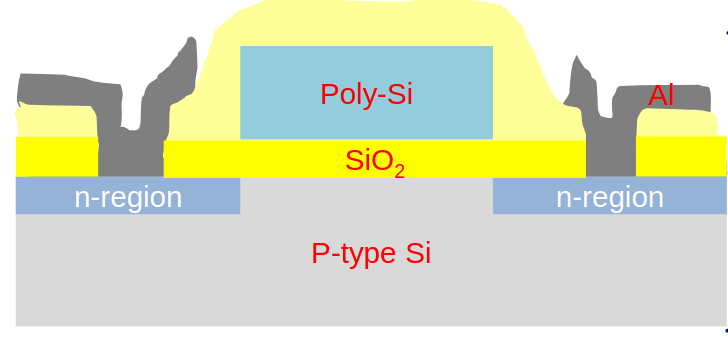
\includegraphics[width=0.95\linewidth]{slice_wafer.png}
  \end{center}
  \caption{Wafer sliced}
  \label{fig:Wafer_slice}
\end{wrapfigure}

It is important to remember that the difference between a NMOS and a PMOS is the type of channel that appears between the drain and the source. Namely in a NMOS we have the appearance of a n-channel (electrons) among a P-type doped silicum.\\

Most schematics of this course are not \textit{up to scale} ! so it is important to remmeber some typical values : 

\begin{itemize}
    \item Wafer diameter \& Thickness:
    \begin{itemize}
        \item 4" : 400 $\mu m$
        \item 8"-12" : 1200 $\mu m$
    \end{itemize}
    \item Thickness of a layer : 1-3 $\mu m$
\end{itemize}

A good comparison for this scale is a single hair which is approximately 75 $\mu m$.

\section{Basic steps of IC fabrication}

We always start from a wafer, either P-type or N-type. Here we will discuss the fabrication of a NMOS type of transistor so we will need a P-type Si wafer.

\begin{enumerate}
    \item \underline{Oxidation :} We deposit a layer of $SiO_2$ by either \textit{growing} or \textit{depositing} it at high temperature.
    \item \underline{Deposition of poly-Silicon :} we will deposit some poly-crystalline silicon using \gls{cvd}.
    \item \underline{$1^\circ$ photoresist :} we use some organic photoresist and to evenly disperse it we will spin the wafer. This will help spreading evenly the photoresist and making it thinner. Many version and purity of this compound exists.
    \begin{itemize}
        \item \textit{Lithography :} we will shine UV light through a mask (why UV ? shorter $\lambda$ so smaller features size possible). After this we will simply etched away the area that were exposed to UV light (so it gets smoother through UV exposure and stay harder otherwise)
    \end{itemize}
    \item \underline{Etching of Poly-Si :} we will use some \textit{dry} (plasma) or \textit{wet} etching and then we remove the rest of photoresist.
    \item \underline{Doping of Source and Drain region :} we send ion at high speed on the wafer (ion implementation) and to repair the damage we "\textit{cook}" it around $900^\circ$. It can easily traverse the thin $SiO_2$ layer but not the poly-Si.
    \item \underline{Wrapping \& Adding contact :}
    \begin{itemize}
        \item \textit{Deposit of Oxide :} again with some \gls{cvd} we put a layer of oxide. This result in unsmooth surface.
        \item \textit{Add photoresist :} then use UV mask and etch at specific spot over the Source and Drain.
        \item \textit{Remove photoresist}
        \item \textit{Add metal :} we do some \gls{pvd}
        \item \textit{Remove metal over the gate :} we don't want any layer of metal over the gate or we will create more unwanted capacitance. So we again use photoresist, UV mask, etch photoresist, etch metal and finally remove the remainder of photoresist.
    \end{itemize}
\end{enumerate}

An important distinction to be made is when we are talking about mask they can be either : 

\begin{itemize}
    \item \textit{Photo mask :} use of a blocking and non blocking UV light mask to make a photoresist compound react or not.
    \item \textit{Etch mask :} the remaining photoresist (after etching of non hardened one) is used as a protective layer to not etch unexposed surfaces.
\end{itemize}

Mass producing and producing in batch is a key to bring down the costs of IC. We can produce a lot quickly and efficiently and with good design we can leave room for error and process variation meaning we can increase yields.

\section{Silicon}

\begin{wrapfigure}{r}{0.5\textwidth}
  \begin{center}
    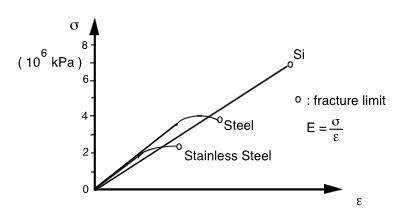
\includegraphics[width=0.95\linewidth]{resistivity_Si.png}
  \end{center}
  \caption{Stress curves for various material}
  \label{resistivity_Si}
\end{wrapfigure}

Silicon is one of the favorite material since it is :

\begin{itemize}
    \item Cheap, strong (and fragile)
    \item 0.001 - 20 $k\Omega/cm$
    \item Stable oxide ($SiO_2$) pretty inert (wow)
    \item various flavors of lattice, Silicon-Crystalline-Silicon, poly-silicon, amorphous silicon (unordered)
\end{itemize}

We can also use some GaAs, Quartz (which is just $SiO_2$ with other things), SiC, $Al_2O_3$. On the figure \ref{resistivity_Si}, we can see how the Silicium can deform under pressure and come back to its original shape without breaking for large values. We can even make some wafer flexible using special processes to make it extra thin.\\

We mostly use crystalline like Silicon even though non-crystalline have become somewhat important in the industry. The doping plays a role regarding the resistivity of the material.

\begin{figure}[H]
    \centering
    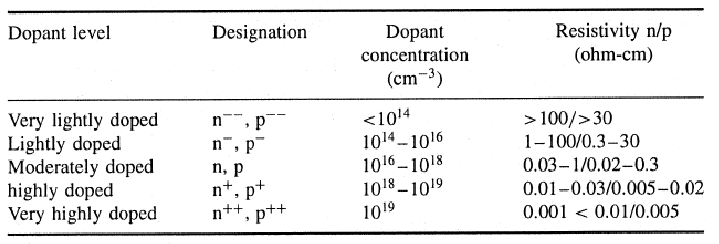
\includegraphics[width=0.75\linewidth]{resistivity_Ohm_Si.png}
    \caption{Resistivity for various doping level}
    \label{fig:resistivity-Si-Ohms}
\end{figure}


\newpage
\begin{wrapfigure}{r}{0.5\textwidth}
    \centering
    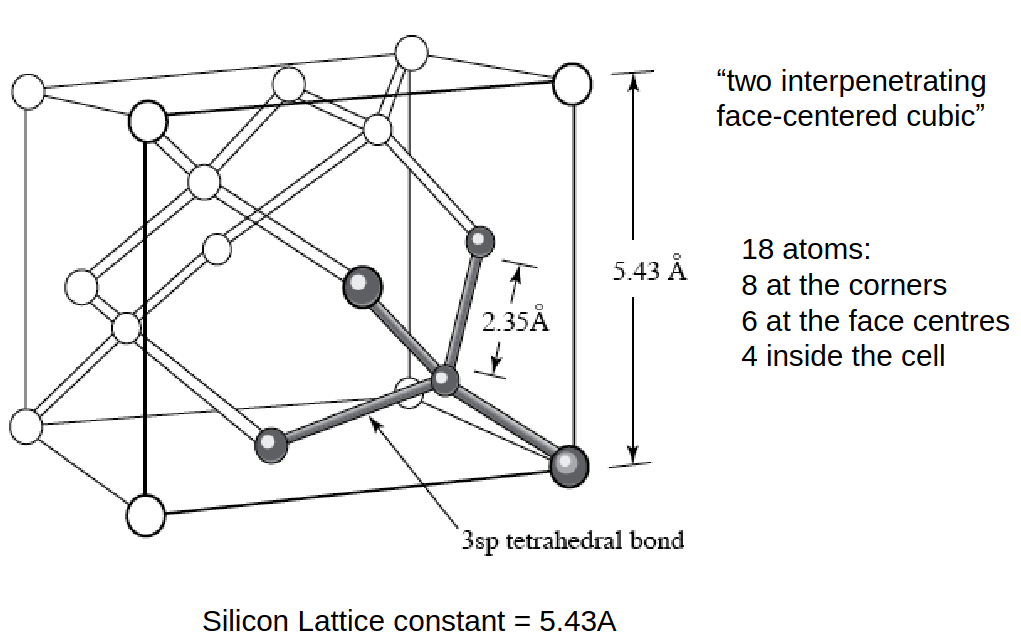
\includegraphics[width=0.95\linewidth]{crystal_si.png}
    \caption{Diamond-like Structure of Si}
    \label{fig:diamond-structure}
\end{wrapfigure}

Silicon atoms have \textit{4 valance electrons} and their \textit{covalent bonds} are in a \textit{pryamid like structure} (\textbf{tetrahedron}). For doping we can use : 
\begin{itemize}
    \item \underline{N-type :} use 5a group : Arsenic, Phosphorous, ...
    \item \underline{P-type :} use 3a group : Boron, Gallium, Aluminum, ...
\end{itemize}

We have 4 atoms completely inside of a unit cell, the 8 ones on the corner are shared with other cell (and count as 1 atom inside cell) and the 6 remaining atoms on the faces are shared with 2 cells (count as 3 atoms inside cell). So we have $4+1+3=8$ atoms inside the cell and the cell volume is $(.543 nm)^3 = 1.6 \cdot10^{-22} cm^3$ which leads to a density of $\frac{8}{1.6 \cdot10^{-22} cm^3} = 5 \cdot 10^{22}$ atoms $/cm^3$.\\
To represent which angles we are viewing a cell, we are using the \textbf{miller indices}. Different orientations of the lattice impact the properties of the transistor due to different lattice form.

\subsection{Miller Indices}

To find the miller indices, we need to first draw a plane and see where it intercepts with any x,y,z axis. If we only intercept the x axis at $a$ then we can write $[1 \quad 0 \quad 0]$ if we normalize $a$ as the \textit{cubic cell constant}.\\
We have various notation each with its own rule:

\begin{itemize}
    \item \underline{$[100]$ :} \textbf{direction} in crystal coordinate
    \item \underline{$<100>$ :} set of \textit{symmetrically equivalent} \textbf{direction} in crystal coordinate
    \item \underline{$(100)$ :} \textbf{plane} \textit{perpendicular} to a direction
    \item \underline{$\{100\}$ :} set of \textit{symmetrically equivalent} \textbf{plane} in crystal coordinate
\end{itemize}

To find the angle between two crystallographic directions we use the equation with the two directions being $[h_1k_1l_1]$ and $[h_2k_2l_2]$ : 
\begin{equation}
    cos(\theta) = \frac{h_1 h_2+k_1k_2+l_1l_2}{\sqrt{(h_1^2+k_1^2+l_1^2)(h_2^2+k_2^2+l_2^2)}}
\end{equation}


\section{Production of wafers}

Single crystal silicon is one of the purest material made artifically  with a purity of $99.999999999$ \%. We have a FCC lattices displaced by $.25$ \r{A} in the 3 directions.

\begin{figure}[H]
    \centering
    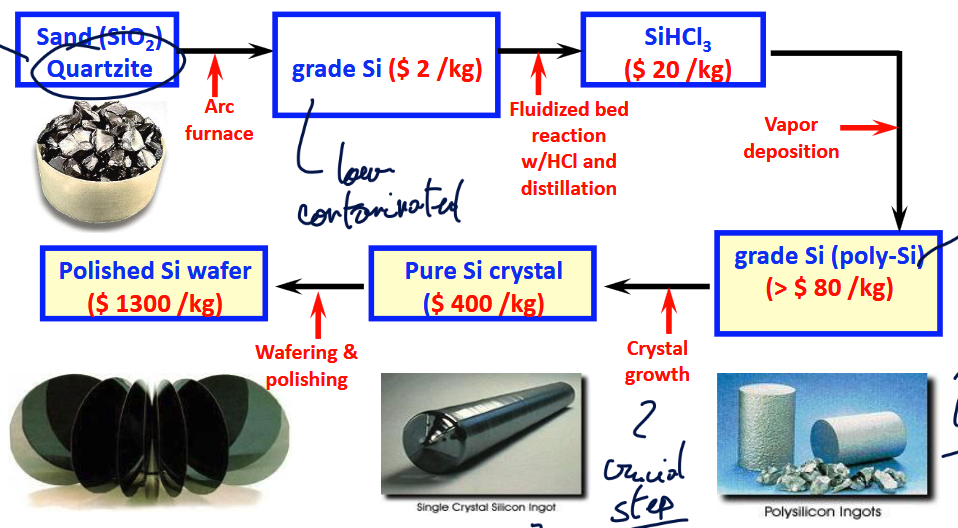
\includegraphics[width=0.75\linewidth]{cycle_si.png}
    \caption{Cycle of Si production}
    \label{fig:si-production-label}
\end{figure}

We can have some defect and non-idealities in the boule. Typically we want a mono-crystalline structure where everything is ordered in the same direction. But we can have :

\begin{itemize}
    \item \underline{Polycrystalline :} multiple pockets named \textbf{grain} (or crystallites) where we find different direction of crystal
    \item \underline{Amorphous :} unorganized structure and random
\end{itemize}

But first, we need to melt this \textit{quartz sand} with carbon at over $1900^\circ$C. We have a purity of over $98$ \%.

\subsection{Wafer processing}

\subsubsection{Czochralski Pulling}

To create the big boule we then use to slice into wafers, we need to use a specific machine. Typically, we need to use a \textit{seed crystal} with a specific orientation which will make sure to give the same orientation to the boule. We dip it and rotate in counter direction the pot and the seed crystal. The rotation speed is important and the diameter is \textit{inversely proportional to the pull rate}. The pull rate is in $mm/min$ and it takes a lot of time to produce just one boule. We need 30 hours to create a 2m boule and another 30 hours for heating and cooling.\\

\subsubsection{Slicing}

To indicate the orientation, we used to add a flat perpendicular to the $<110>$ direction but now we simply use a notch. We mostly use the $<100>$ with a precision of $\pm 0.5^\circ$ and sometimes we use the $<111>$ with $2^\circ-5^\circ$ off axis.\\ 

The cutting is done with wires coated with diamond and we have one feeder spool and another one that takes the used wires.

\subsubsection{Wafer after treatment}

\begin{enumerate}
    \item \textbf{Lapping} grind both sides, flatness around $2-3 \mu m$, removes $20\mu m$ per side.
    \item \textbf{Edge Profiling}
    \item \textbf{Etching} chemical etch to remove \textit{surface damage}, removes $20\mu m$ per side.
    \item \textbf{Polishing} chemi-mechanical polish, using a slurry composed of $Si O_2$ and some $NaOH$, removes $25\mu m$ per side. Nice mirror finish.
    \item \textbf{Cleaning and Inspection}
\end{enumerate}

\subsubsection{Crystal Orientations}

\begin{figure}[H]
    \centering
    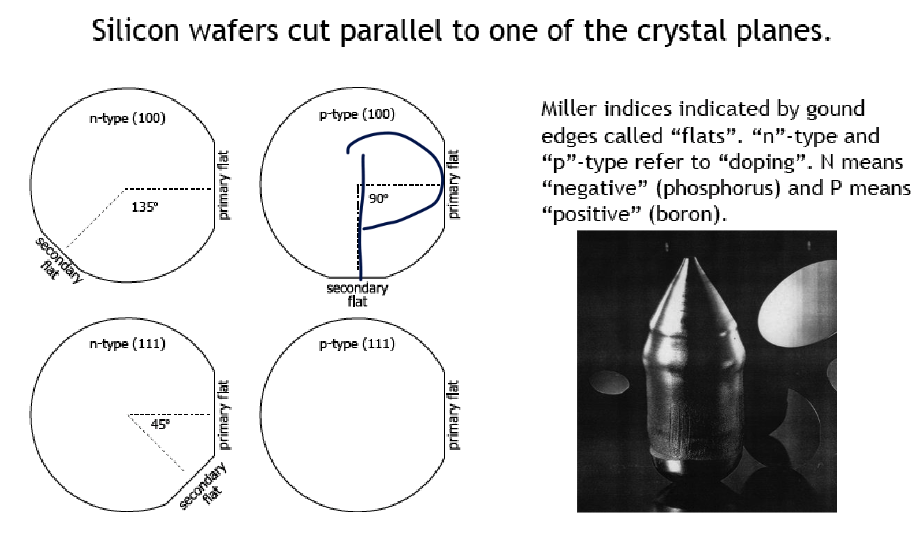
\includegraphics[width=0.75\linewidth]{crystal_orientation.png}
    \caption{Crystal orientation}
    \label{fig:crystal-orientation-label}
\end{figure}

\newpage
\begin{wrapfigure}{r}{0.55\textwidth}
    \centering
    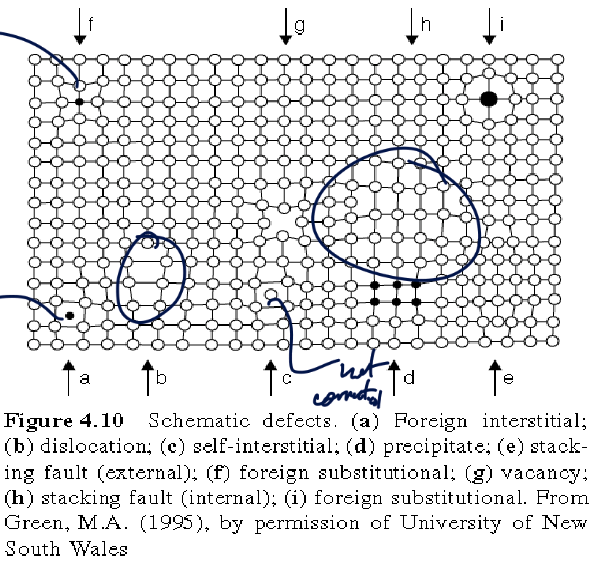
\includegraphics[width=0.95\linewidth]{silicium_non_idealities.png}
    \caption{Silicium non idealities}
    \label{fig:si-non-idealities-label}
\end{wrapfigure}

But nowadays, we are using notches and not really using fully doped wafer. We are doping locally the wafer. A notch indicates a $<100>$ n-type wafer.\\ 

We are processing the wafers in batches of 12 or 24 and they sit on a glass tray (quartz boat) so the support doesn't melt. We will oxidize the wafer to dope it which will tint the wafer. The color of the tint can be used to see what type of doping it is and how doped it is using some optics properties.\\

All those issues will lead to non-functional dies. We usually put some dye on those to clearly and visually indicate if they are good or not. We can't use the dies that are too close to the edge (\textit{edge exclusion} 6 mm for 100-mm diameter wafers).\\

For this reason, we are wanting to use smaller chips to increase the yield. There exists an ideal size that is related to the yield and packaging cost. Now we have an optimum around $13 cm^2$.

\subsubsection{Packaging}

To do some packaging we need to dice the wafer, then use a pick and place arm and finally add some wire (wire bonding) from the chip and its pad to the housing of the chip.


\section{Cleanroom}

\begin{figure}[H]
    \centering
    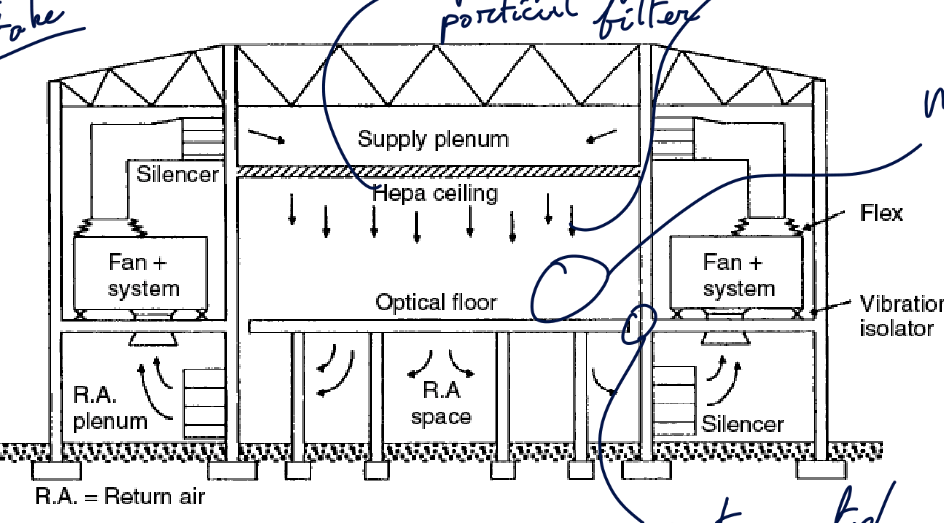
\includegraphics[width=0.7\linewidth]{cleanroom.png}
    \caption{Cleanroom}
    \label{fig:cleanroom-label}
\end{figure}

The purified air comes from the ceiling where it needs to go through some \textit{HEPA} (High efficiency particulate air) filter in the ceiling. We will usually only put one under the arrival of the air and over the crucial equipment to reduce cost.\\

We have various class where each number indicates the amount of particles $>0.5\mu m$ in a cubic foot of air :

\begin{itemize}
    \item Class 10000 : PCB, electronic packaging, medical devices
    \item Class 1000 : MEMS, electronic packaging, hard disk drives
    \item Class 100 : MEMS, RF/Photonic ICs
    \item Class 10 : ICs
\end{itemize}

We also use the ISO standard : 

\begin{table}[H]
    \centering
    \begin{tabular}{|c|c|c|c|c|c|c|c|}
    \hline
    Class & FS209 & 	0.1 $\mu m$ &	0.2 $\mu m$ &	0.3 $\mu m$ 	&0.5 $\mu m$ 	&1 $\mu m$ &	5 $\mu m$\\
    \hline
    ISO1& 	&10& 	2 	  	&&&&\\  	  	 
    \hline
    ISO2& 	&100 &	24& 	10& 	4 	& & \\  	 
    \hline
    ISO3& 1	&1,000 	&237 	&102 	&35 &	8 	 & \\
    \hline
    ISO4& 	10&10,000 &	2,370 	&1,020 &	352 	&83 	&\\
    \hline
    ISO5& 	100&100,000 	&23,700 	&10,200 	&3,520 	&832 &	29\\
    \hline
    ISO6 &	1,000&1,000,000& 	237,000 	&102,000& 	35,200& 	8,320 	&293 \\
    \hline
    ISO7 &	10,000& & & 	&  	  	352,000& 	83,200 	&2,930 \\
    \hline
    ISO8 &	100,000& & 	&&  	  	3,520,000& 	832,000 &	29,300\\
    \hline
    ISO9 &	& & 	 && 	  	35,200,000& 	8,320,000& 	293,000\\
    \hline
    
    \end{tabular}
    \caption{Comparison of ISO and FS209 standard}
    \label{tab:my_label}
\end{table}

The cost in chips is due to the lithography where one chip can go through 10 cycles and the more cycle we have the more expensive it is.

\chapter{Lithography, photoresists, exposure, development}

When we do the lift-off we can either use \textit{positive} photo-resist or \textit{negative} photo-resist. In positive, it is like usual, the photo-mask is used to protect area that shouldn't be etched away. But some compounds are not easy to etch. So sometimes, it is better to use negative process to first deposit the photo-resist and then do the blanket deposition of the compound. Then the lift-off is easy. We need some special trapeze shape that lays on the smaller side for this process. 

\section{Lithography: basic steps}

The goal behind photolitography is to transfer a pattern into structure in a thin layers. By repeating this operation multiple time we can create some intricate and complex integrated circuits.

It mostly revolves around 3 major steps:

\begin{enumerate}
    \item \underline{Resist coating:} we deposit a light sensitive photoresist
    \item \underline{Exposure:} we expose some part of it through a structural mask
    \item \underline{Development:} we remove the photoresist
\end{enumerate}

Photoresist can be used in many many ways. When we etch away compounds we usually have some \textit{undercut} which can be a structural problem.

\subsection{Clean wafer}

We first remove the particle with some rinsing in isopropanol, ultrasonic and megasonic baths. To remove the organic particle we can use some Piranha solution. To remove the metal traces that could diffuse into the wafer, we can do some classic RCA clean, this step is needed before high-temperature steps. RCA also removes ions that may be in the substrate.

\subsubsection{RCA-clean}

\begin{enumerate}
    \item Removal of the organic contaminants (organic + particle clean)
    \item Removal of thin oxide layer (oxide strip, optional)
    \item Removal of ionic contamination (ionic clean)
\end{enumerate}

\subsubsection{IMEC clean}

The RCA-clean is quite an aggressive process and requires lot of chenical products. The IMEC clean is a bit more nature friendly and uses drying to force the particules to stay in the bath and not on the wafer.

\subsection{Anti-reflective coating and adhesion promoter}

We use some Hexamethyldisilazane that will remove OH groups from the surface making the wafer hydrophobic and thus photoresist-philic (since photoresists are apolar).

\begin{enumerate}
    \item \textbf{TARC:} Top-side Anti Reflective Coating.
    \begin{itemize}
        \item Spin coated on top of photoresist
        \item Easier process
        \item Inferior performance
    \end{itemize}
    \item \textbf{BARC:} Bottom side Anti-Reflective Coating.
    \begin{itemize}
        \item Deposited below photoresist layer
        \item Better performance
        \item Longer processing (plasma-etched)
    \end{itemize}
\end{enumerate}

\subsection{Coat with photoresist}

We can have positive or negative photoresist where:

\begin{itemize}
    \item Positive: exposed area gets softer and easier to etch
    \item Negative: exposed area gets harder and harder to etch
\end{itemize}

Spin coating is a process where we depose some droplets and spin the wafer. Spinning it at a slow speed will spread the compound equally and then we finish it off by spanning faster. It is a pretty good and convenient way to coat a wafer's surface. But we can have some bumps around the side of the wafer (edge bead) and the way steps are coated is not always perfect.

\subsubsection{Resist spinning}

We have some empirical equations for the thickness, and we spin with a force of around 5 NM.

\begin{equation}
    T = \frac{K \cdot C^\beta \cdot \eta^\gamma}{\omega^\alpha}
\end{equation}

Where $K$ is the calibration constant, $C$ polymer concentration in gram per 100 mL, $\eta$ intrinsic viscosity, $\omega$ rotation per minute. The exponents are empirically determined.

We can also remove those edge bead in the process. But this doesn't solve the issue of uneven coating around steps of the wafer.

\subsubsection{Spray coating}

We have two nozzles where one will be used as the developer and the other one is to rinse the wafer. It provides a smoother step coverage and is widely used in MEMS devices.

\subsubsection{Other methods}

We can also think about dip coating, laminating dry films of photoresist, ...

\subsection{Soft Bake}

It is used to remove the solvents in the resist. It is non-sticky, improves resolution, improves the strength of resist. But we shouldn't bake too high too long or we would cause the embrittlement and make the removal harder.

\subsection{Exposure}

There exists 5 exposure methods:

\subsubsection{Lithography}

We expose the resist to UV light through a mask. We have to align the mask precisely, it can be done manually for older technology. The smaller we go the more expensive a mask is and we have more and more layers.

\subsubsection{Limits}

The main issue is the diffraction effects. Indeed, we have effects where we could have some destructive or constructive waves that can be unforseen. That's why some mask can have special patterns that will result in the desired effect.

Those special patterns are Phase Shifting Mask where we will have some special pattern to change the phase.

The process of making the wafer reflective can sometimes lead to create some standing waves. Those standing waves can lead to uneven development and rippled sidewalls. A solution for this is to use \gls{arc} or post exposure bake. This can also lead to linewidth variations due to reflection.

\begin{figure}[H]
    \centering
    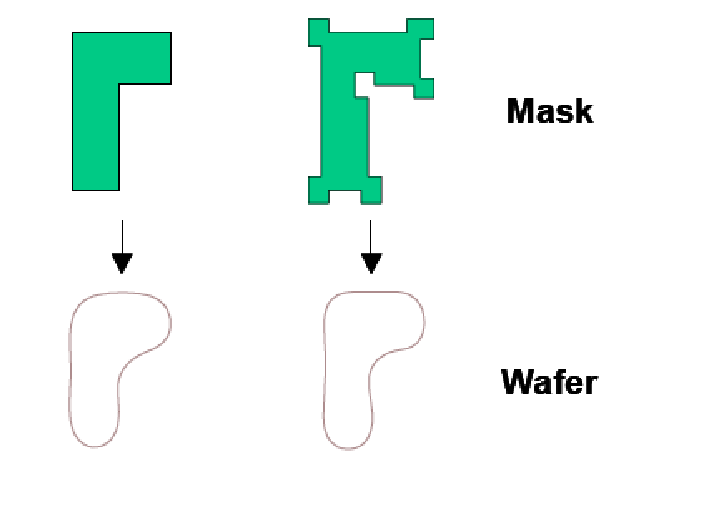
\includegraphics[width=0.5\linewidth]{OPC.png}
    \caption{Optical Proximity Correction}
    \label{fig:enter-label}
\end{figure}

\subsection{Different printing techniques}

\begin{figure}[H]
    \centering
    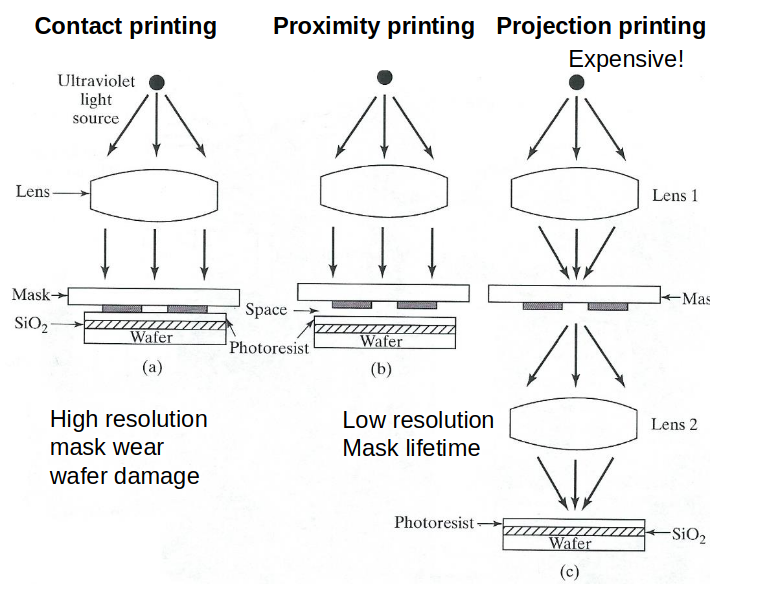
\includegraphics[width=0.65\linewidth]{printing_techniques.png}
    \caption{Printing techniques}
    \label{fig:enter-label}
\end{figure}

Usually we use stepper to print successively a pattern on the wafer.

\subsubsection{Projection printing}

We concentrate and project on the wafer, There is a few key metrics such as:

\begin{itemize}
    \item \underline{Numerical Aperture:} $NA = n sin(\theta)$
    \item \underline{Critical Dimension:} $CD = kl \frac{\lambda}{NA}$
    \item \underline{Depth of Focus:} $DOF = k_2 < 1$
\end{itemize}

The depth of focus is an indicator to know when it is no longer good for focus.

\begin{figure}[H]
    \centering
    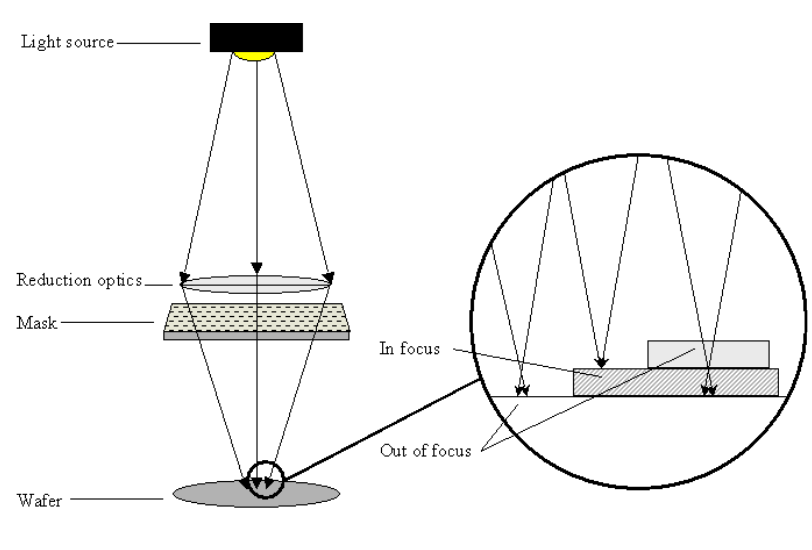
\includegraphics[width=0.5\linewidth]{DOF_effects.png}
    \caption{DOF effects}
    \label{fig:enter-label}
\end{figure}

\subsection{Light source}

Another important parameter we can play is the light source. Back then, we used mercury bulbs for most lithographic work. It was a good enough and pretty cheap UV source. But it would produce various line of UV. So we had to use some filter to get only a specific wavelength.

\begin{table}[hbt]
\centering
\begin{tabular}{l l l}
%\hline
\textbf{Source} & \textbf{Wavelength (nm)} & \textbf{Name} \\
\hline
Hg arc lamp     & 436 (blue)               & g-line         \\
                & 405 (violet)             & h-line         \\
                & 365 (UV)                 & i-line         \\
                & 248                      & DUV            \\
%\hline
KrF excimer laser & 248                   & DUV            \\
%\hline
ArF excimer laser & 193                   & DUV            \\
%\hline
F\textsubscript{2} excimer laser & 157     & DUV (vacuum UV)\\
%\hline
plasma          & 13                       & EUV (long x-ray) \\
%\hline
\end{tabular}
\caption{Wavelengths of light sources used in photolithography}
\end{table}

The main attract to use lower wavelength light source is to be able to draw better and smaller features. A good way to circumvent this rat race is to use multiple mask to produce one result. So we can use multiple ask with more spaced out features which simplifies amd relax constraints of the problem.

\begin{enumerate}
    \item Double patterning: Litho-Etch-Litho-Etch (LELE)
    \begin{itemize}
        \item First technique introduced, reduces $k_1$
        \item More costly as it doubles the amount of mask, need a hard mask, possible overlay issues
    \end{itemize}
    \item Double patterning: Self-Aligned Double Patterning (SADP)
    \begin{itemize}
        \item Solution to the overlay issue of LELE's masks self aligning
        \item Single lithography step, need to use an additional block or cut mask to remove unwanted material
        \item Complicated to design masks, process intensive
    \end{itemize}
    \item Double patterning: Litho-Freeze-Litho-Etch (LFLE)
    \begin{itemize}
        \item Less complicated process than LELE, increased throughput, no need for hard mask.
        \item Dependent on development of freezing process, freezing cam cause issues in the lines.
    \end{itemize}
    \item Double patterning: self-aligned quadruple patterning (SAQP)
\end{enumerate}

\subsection{EUV}

This is the hot new trend in the industry (ASML has the technology but maybe huawei who knows). There has been prototypes since 2017 that can do $13.5$ nm and NA $0.33$. It doesn't not have lenses but only mirrors as we can't focus EUV light like this.

\subsubsection{Issues}

We need to use some Bragg reflector that have an alternating thickness of 2 nm of Mo and Si. It can only reflects $70\%$  per mirror, so we need a quite intense light source or we won't have anything coming to the wafer.

\subsubsection{Photo vs E-beam lithography}

With E-beam lithography, we can be really accurate and not use any mask, it comes at the disadvantage to slower processes. So we use E-beam to create the mask for photo-lithography.

An issue is the scattering of the electron inside the wafer, it can also go further than expected and in a random pattern.

\subsection{Post exposure bake}

It can help with wrinkles in the side wall. Baking can smooth things out and is quite standard for positive resist. Can also enhance crosslinking in negative resist.

\subsection{Develop - wet process}

Development is a wet chemical process as the wafer is immersed in developer and rinsed and dried afterwards. We can also spray the developer on the wafer as it spins but can be used and then dried. We can use the spraying nozzle techniques.

\subsection{Hard bake}

Sometimes used to improve etch resistance of resist. But it can causes the softer resists to reflow.

\subsection{Etching, metal deposition, ion implantation, ...}

See next chapters

\subsection{Remove photoresist}

To remove the pohotoresist, we can either go for wet etching with some specialized solutions or acetone, NaOH, ...

We can also opt for O2 plasma etching.

\chapter{Deposition: \gls{pvd}, \gls{cvd}, Epitaxial growth, \gls{ald}}

To deposit a thin film layer we can use some \gls{pvd} with evaporation or sputtering. Another method is \gls{cvd} that uses thermal, low pressure and plasma enhanced (electrons stripped away from atoms).\\

With evaporation (heat + vacuum) we can reach a growth rate of $0.1-1 nm/s$. With sputtering (vacuum + plasma) we have a rate of $1-10nm/s$.

\section{\gls{pvd}}

\subsection{Vacuum}

\begin{wrapfigure}{r}{0.5\textwidth}
    \centering
    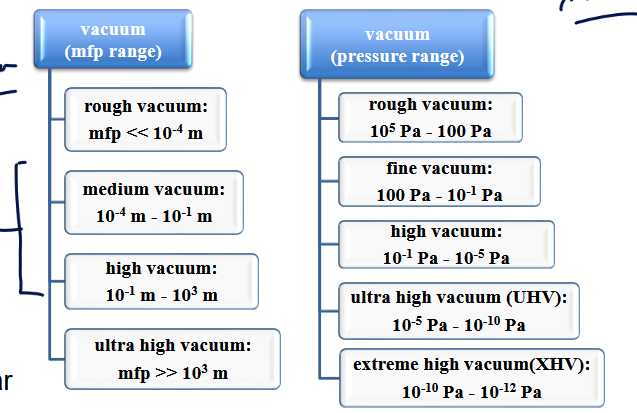
\includegraphics[width=0.95\linewidth]{vacuum.png}
    \caption{Vacuum grade}
    \label{fig:vacuum-label}
\end{wrapfigure}

To realize deposition we need certain grade of vacuum. They are graded based on their \gls{mfp}. It indicates how far can a molecule travel before hitting an other one. There is an equivalency between \gls{mfp} and the pressure in the environment. 

The roughing pumps are simple a valve that rotates and will take out the air. But it is not the purest form of vacuum.\\

High vacuum diffusion pump use some oil. The oil is heated up and will vaporize, then when it gets cooled down it will take with them molecules. The pressure at the bottom is higher and so we can simply use a pump to take those extra molecules the oil vapor captured.

In a turbomolecular pump we are using some stator and rotor blades that are inclined in such way that when a molecules strike the turbine blade it will bounce and slowly travel to the bottom of the pump.

There is also cryogenic pump that is a mix of previously introduced vacuum pumps.

\begin{figure}[H]
    \centering
    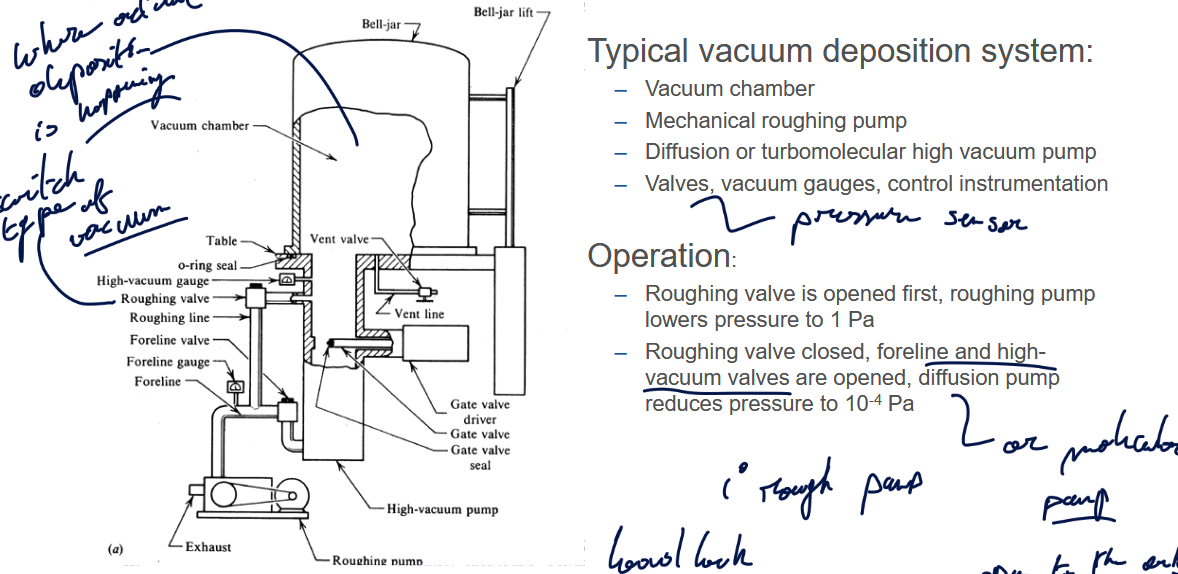
\includegraphics[width=0.75\linewidth]{Vacuum_PVD.png}
    \caption{Typical system for \gls{pvd}}
    \label{fig:PVD-label}
\end{figure}

\subsubsection{Pirani Gauge ($> 10^{-3}$ mbar)}

It is based on a \textit{weathstone bridge}. We will use a platinum wire that is pretty linear and will get heat up, the way this heat transfer occur depends on the pressure and is lower at lower pressure. So there is a direct link with pressure, heat and finally resistor which is easy to measure with such bridge.

\subsubsection{Ion gauge ($< 10^{-2}$ mbar) }

The filaments will create a \textit{space-charge} of free electrons. The electrons are attached by the positive grid and the collisions with the gas atoms will create Ion which can be measured.

\subsection{Evaporation}

Now, we want to actually vaporize and create thin film on our wafer to grow all sorts of oxide, metals, polysilicon,  ... There is two ways to do it :

\begin{enumerate}
    \item Resistance heating evaporation : 
    \begin{itemize}
        \item We have the crucible (holder of the compound) and the target (wafer) that gets heated
        \item Only low melting temperature point metals (or it gets too hard)
    \end{itemize}
    \item Electron beam evaporation :
    \begin{itemize}
        \item We use some electron beam to strike the material that will get \textit{sublimate} (not a melting)
        \item We cool the crucible down and it doesn't need to be as pure as with heated method
        \item Good for high melting point metals
    \end{itemize}
\end{enumerate}

\begin{figure}[H]
    \centering
    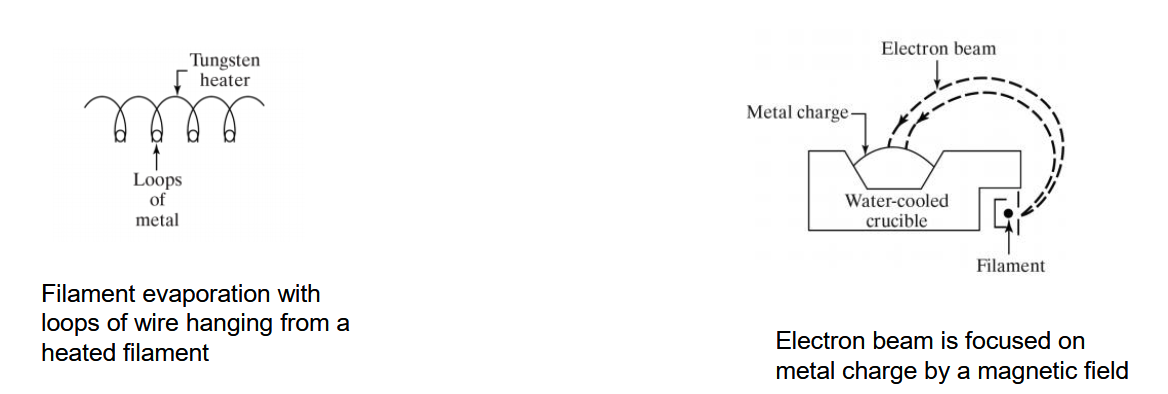
\includegraphics[width=0.85\linewidth]{evaporation_method.png}
    \caption{Evaporation techniques}
    \label{fig:evap-label}
\end{figure}

\subsubsection{Coverage issues}

Due to the radiating pattern from the crucible to the target, we will have discontinuity on the wafer which is not acceptable for traces or oxide. So we will gently spin the target to slightly change the momentum and so atoms will strike the sidewall. We also heat up the substrate to further help the step coverage.

\begin{figure}[H]
    \centering
    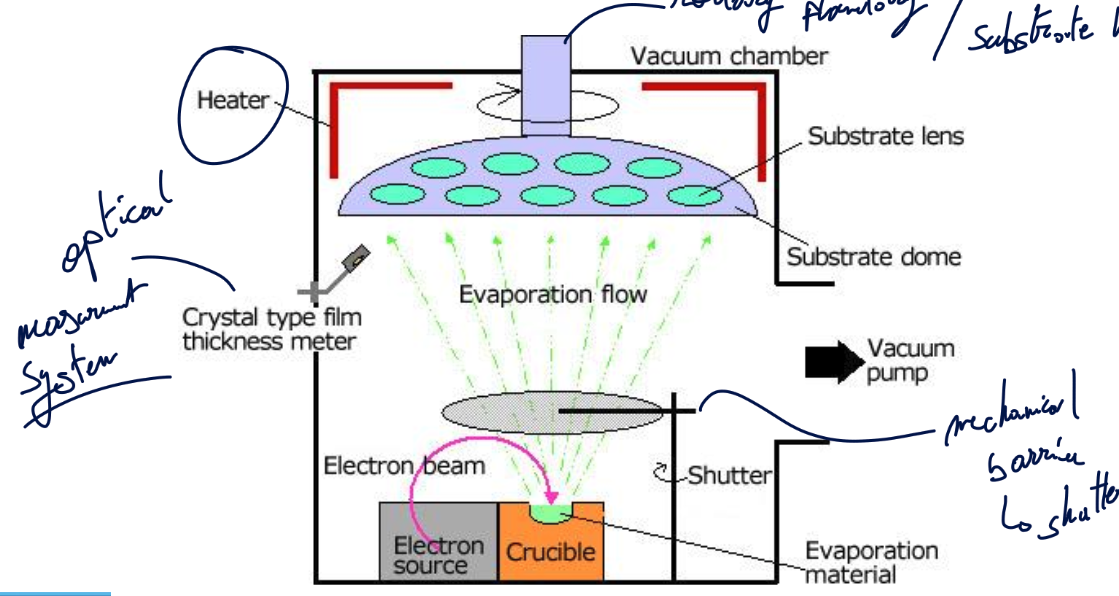
\includegraphics[width=0.5\linewidth]{config_PVD.png}
    \caption{Configuration for \gls{pvd}}
    \label{fig:pvd-conf-label}
\end{figure}

\subsection{Plasma}

Plasma is a low pressure gas where a high energy field is used for ionization creating a large number of ions and free electrons. So we rip electrons of the nuclei and this happens in a vacuum. Plasma contains an equal concentrations of ions and electrons. Electric potential is approximately constant inside the plasma. We are using weak plasma so mostly neutral atoms/molecules.

\begin{figure}[H]
    \centering
    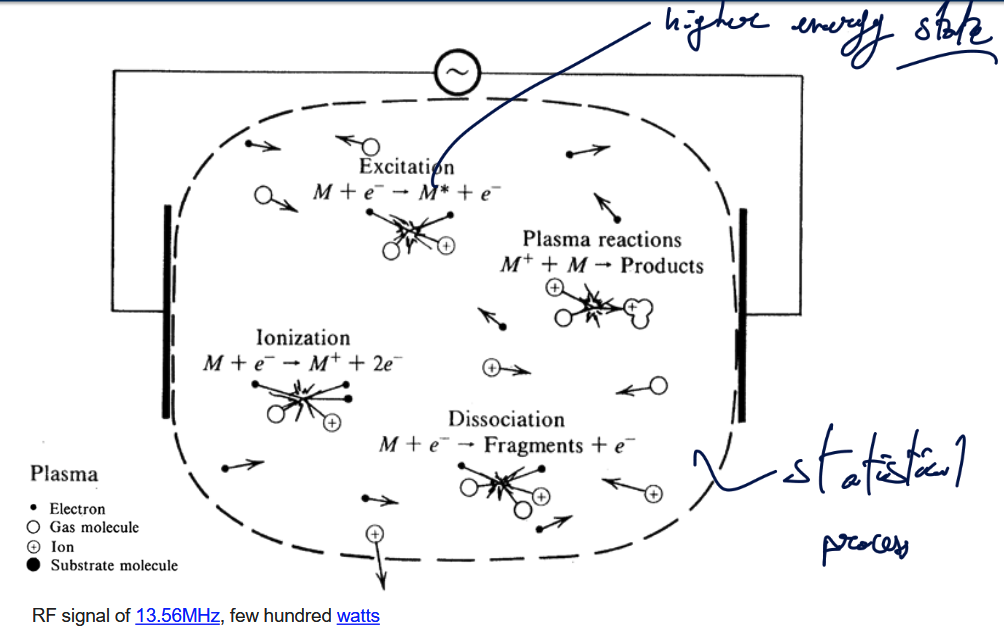
\includegraphics[width=0.51\linewidth]{plasma.png}
    \caption{Plasma using sputtering}
    \label{fig:plasma-sputtering-label}
\end{figure}

So the ions of the plasma will strike the target releasing them and letting them go onto the wafer. We talk about a \textbf{sputtering yield} which indicates $S = \text{\# of ejected target atoms} / \text{incoming ions}$ and it is usually $0.1<S<30$.\\

For example we can use a plasma of $N_2$ and a $Ti$ target that will create a thin film layer of the substrate of $TiN$.\\

Using sputtering can be quite beneficial especially for multi-components thin-films. It is also better for lateral thickness uniformity. We have a superposition of multiple point sources.

\section{\gls{cvd}}

The idea here is to use some chemical reaction to go from a gas phase to a solid phase. Typically we will use a sort of boundary layer which will trigger a reaction and deposit on the wafer. We need to remember that \textit{natural} chemical reaction are trigger when we mix different molecules that will reach a higher state of energy and will tend to a lower state of energy. If we want to reverse this reaction we need to give the same amount of lost energy.

\begin{table}[hbt]
    \centering
    \begin{tabular}{|l|l|c|l|}
        \hline
        \textbf{Material/method} & \textbf{Source gases} & \textbf{Temperature} & \textbf{Stability} \\ 
        \hline
        \gls{lto}          & SiH$_4$ + O$_2$       & 425$^\circ$C  & Densifies \\ 
        \gls{hto}          & SiCl$_2$H$_2$ + N$_2$O & 900$^\circ$C  & Loses Cl \\ 
        \gls{teos}         & \gls{teos} + O$_2$         & 700$^\circ$C  & Stable \\ 
        \gls{pecvd} OX     & SiH$_4$ + N$_2$O     & 300$^\circ$C  & Loses H \\ 
        \gls{lpcvd} poly   & SiH$_4$              & 620$^\circ$C  & Grain growth \\ 
        \gls{lpcvd} a-Si   & SiH$_4$              & 570$^\circ$C  & Crystallizes \\ 
        \gls{lpcvd} Si$_3$N$_4$ & SiH$_2$Cl$_2$ + NH$_3$ & 800$^\circ$C  & Stable \\ 
        \gls{pecvd} SiN$_x$ & SiH$_4$ + NH$_3$     & 300$^\circ$C  & Loses H \\ 
        CVD-W        & WF$_6$ + SiH$_4$     & 400$^\circ$C  & Grain growth \\ 
        \hline
    \end{tabular}
    \caption{Deposition methods, source gases, temperature, and stability.}
    \label{tab:deposition_methods}
\end{table}

There is many chemical reactions showed in the course so check out page 40-45. When we grow an oxide or anything, we can either be \textbf{mass transport limited} (velocity of the molecules saturate) or \textbf{surface reaction limited} (the surface isn't heated enough and the reaction isn't going well).

\subsection{Reactor}

\begin{figure}[H]
    \centering
    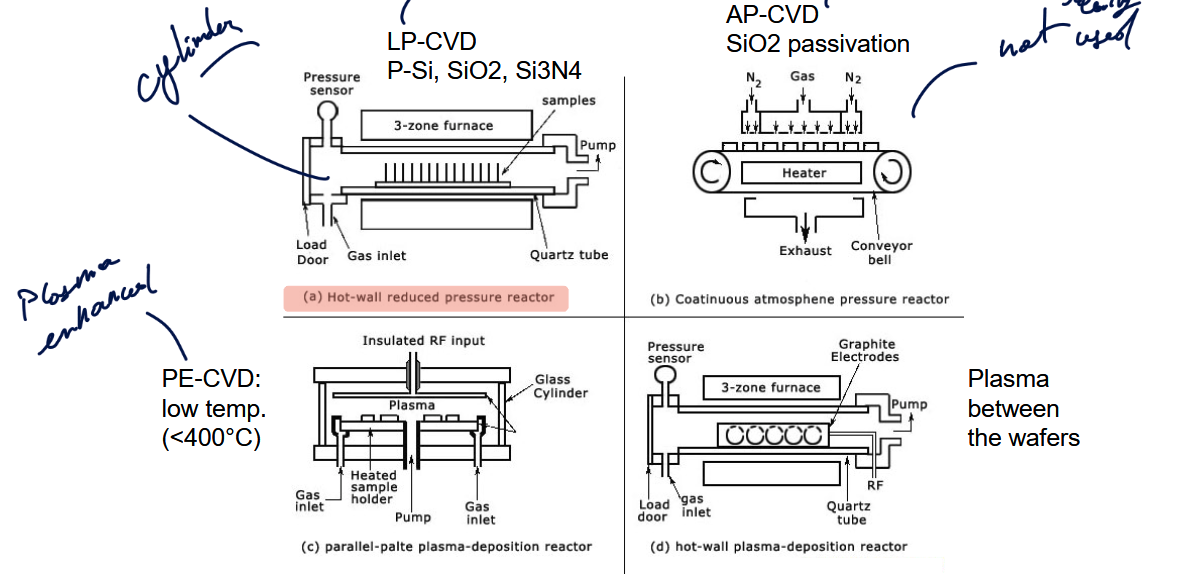
\includegraphics[width=0.85\linewidth]{reactor.png}
    \caption{CVD Reactors}
    \label{fig:cvd-reactors-label}
\end{figure}

\subsubsection{1. APCVD - Atmospheric Pressure}

It is pretty simple, we put the wafer on a conveyor belt that heats up the wafer. We use some ozone and \gls{teos} gas.

\subsubsection{2. \gls{lpcvd} - Low Pressure}

We can stack the wafer vertically so keep them in the boat as we insert them in the furnace. It needs a pressure of $0.1-2$ Torr and it needs high temperature and has a slow growth rate. It is ideal for batch processing.

\subsubsection{3. \gls{pecvd} - Plasma Enhanced}

We induce plasma in the gas by using some RF. We need some inert and process gas and the wafer needs to spin and be heated. This result in better step coverage and needs relatively lower temperature while having a high deposition rate.

\begin{figure}[H]
    \centering
    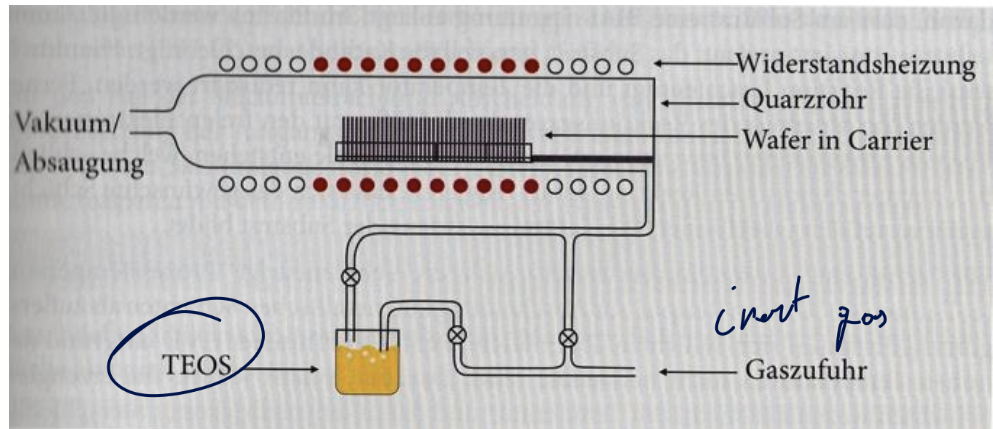
\includegraphics[width=0.65\linewidth]{pecvd.png}
    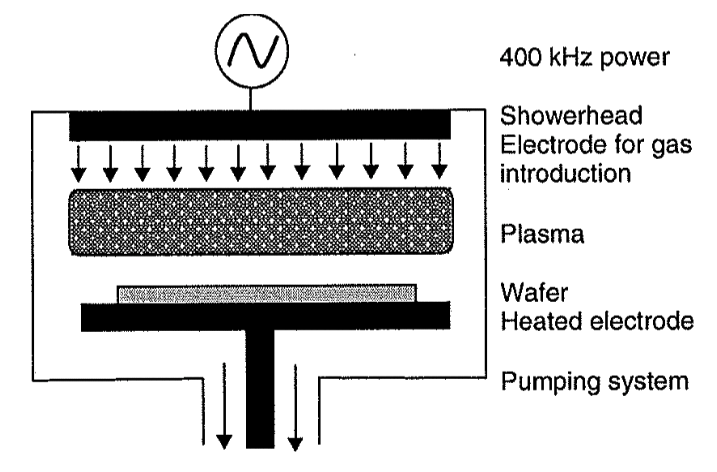
\includegraphics[width=0.33\linewidth]{PECVD_reactor.png}
    \caption{PECVD diagram}
    \label{fig:pecvd-label}
\end{figure}

At higher temperature the deposition pattern will create bigger "\textit{blobs}" compared to lower temperature deposition.

\subsection{Epitaxial growth}

\begin{wrapfigure}{r}{0.5\textwidth}
    \centering
    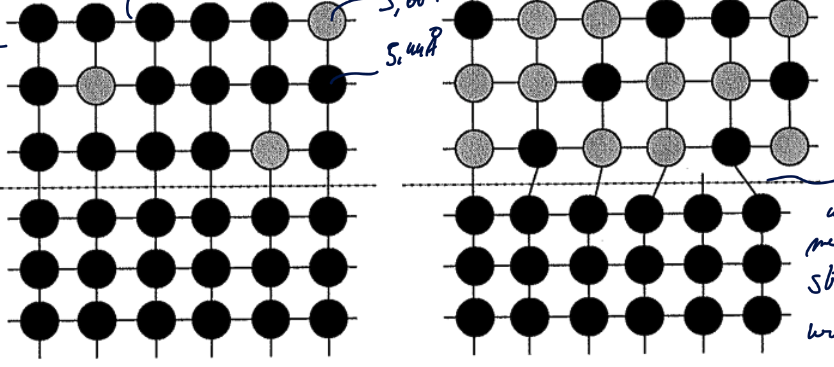
\includegraphics[width=0.95\linewidth]{mechanical_stress_epitaxy.png}
    \caption{Epitaxy stress}
    \label{fig:epitaxy-stress-label}
\end{wrapfigure}

We can grow some layer with the epitaxial technique. We can have : 

\begin{itemize}
    \item Homo-epitaxy : independent doping on a high-conductive substrate
    \item Hetero-epitaxy : the difference in $a$ size could create some mechanical stress
\end{itemize}

Some more advanced and recent epitaxy technique have been developed such as \gls{mbe}. With this new method we can deposit some complex stack of material on our wafer. It is still in development and so there is not yet a wide industry adoption of industrial workstation.

\subsection{\gls{ald}}

With this method we can literally deposit \textbf{1 layer of molecules} at a time ! We use some cycle consisting of a sequential precursor gas pulses. It will produce a monolayer of gas on the substrate. Then a second precursor gas is introduced which reacts with the monolayer and will result into another monolayer on top.

\begin{figure}[H]
    \centering
    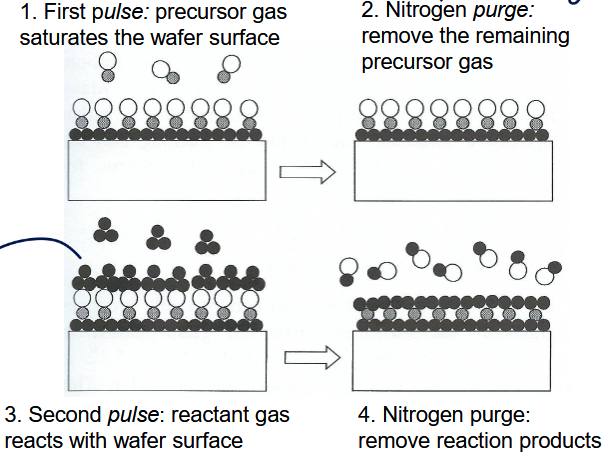
\includegraphics[width=0.65\linewidth]{ALD_cycle.png}
    \caption{\gls{ald} process of pulsed mode}
    \label{fig:ALD-pulsed-mode-label}
\end{figure}

\gls{ald} is a \textit{self-limiting} process so only one layer will be deposited at a time. It is similar to \gls{cvd} but we have 2 major steps to diffuse the precursor gas not at the same time. We usually use Nitrogen or Argon as a \textit{purge gas} which will "\textit{clean}" unwanted atoms. This 2 cycles will help to avoid some \textit{parasitic} deposition like in \gls{cvd}.

It is also pretty good at making \textit{trenches} which is usually a FoM. We usually compare width opening/depth. This value ranges from $20$ to $100$.

\subsection{Deposition from the liquid phase}

\subsubsection{Electroplating or galvanic deposition}

Thick conductor layers, high aspect ratio metallization. For this method, we will use an anode and a cathode. We will use the reduction of $Cu$,$Ni$ or $Au$ typically onto the wafer (used as a cathode). We have a pretty fast growth rate of $0.1-10 \mu m/min$.

It is a good solution to create \textit{through-silicon vias} and do some IC interconnects which is gaining more and more popularity lately.

\subsubsection{Electroless deposition} 

Selective metallization. We can have a growth rate of $100nm/min$. For intereconnect between IC we can use the \textit{damascene technique} :

\begin{figure}[H]
    \centering
    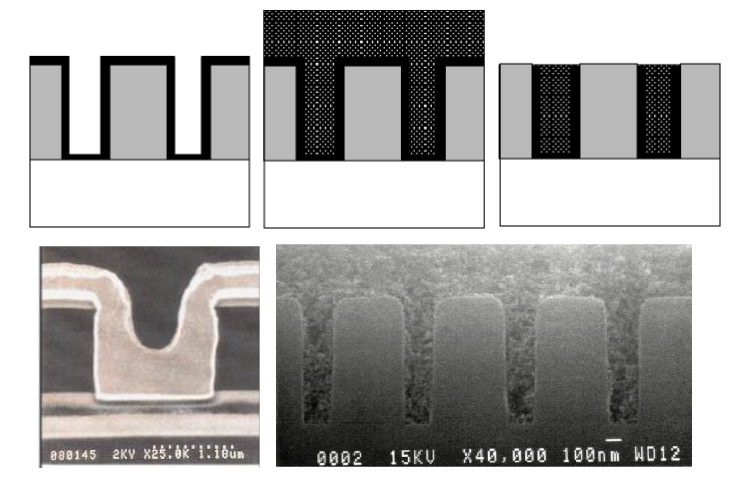
\includegraphics[width=0.5\linewidth]{damascene_technique.png}
    \caption{Damascene technique}
    \label{fig:enter-label}
\end{figure}

\subsubsection{Spin coating}

Photoresists, thick polymer layers, spin-on glasses. Usually we start at a slower speed to have the right amount of photoresist everywhere on the glass then we finally spin it around $5000 rpm$ which will cause \textit{partial drying via evaporation}.

\subsubsection{Sol-gel}

Porous dielectrics, thick and complex materials.

\section{Measuring the thickness}

To measure the thickness of the layer we can :

\begin{itemize}
    \item Mechanical method : we use a needle that will check the thickness. It is not the most precise method.
    \item Optical method : 
    \begin{itemize}
        \item Reflectometry : we need the layer to not be totally opaque and we will measure the various wave that comes out of the wafer. We need to use small die and we can measure from $10nm$ to $50\mu m$.
        \item Elipsometry : it works with the polarization of light and can measure up to $100\mu m$.
    \end{itemize}
\end{itemize}

\chapter{Oxidation, wet, dry}

\begin{wrapfigure}{r}{0.5\textwidth}
    \centering
    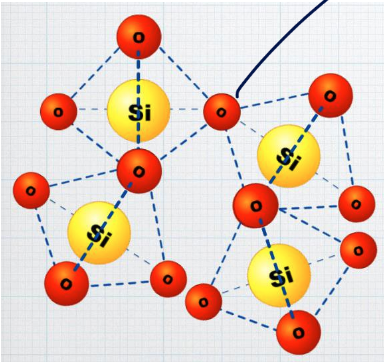
\includegraphics[width=0.95\linewidth]{sio2_structure.png}
    \caption{Structure of $SiO_2$}
    \label{fig:sio2-structure-label}
\end{wrapfigure}

Sand is an abundant material that contains $SiO_2$ or Silicon dioxide. It is the main component of glass, optical fibers and we can find a crystalline structure of $SiO_2$ in quartz.

It has a \textit{tetrahedral arrangement} with one silicon bonded to four oxygen atoms. We can see how most of oxygen atoms will be bonded with $Si$ atoms making the terahedra shape joined at corner. We call those atoms the \textit{bridging atoms}. Not all oxygen atoms will be bonded to two $Si$, we call them the \textit{non-bridging atoms}. The density of those non-bridging atoms determine the quality of the oxide.

They are not always aligned in such regular manner, it can be random making some \textit{amorphous structure}. If there is no non-bridging atoms, then

In microelectronic, we use thin layers of pure $SiO_2$ and they are amorphous. The density is about $2-2.3 gm/cm^3$, $\varepsilon_r = 3.9$ (frequency dependent), $n=1.5$ optical index. The breakdown voltage is $> 10^7 V/cm$ which is the main reason why we need to lower $V_{DD}$ as the thickness of the gate is getting smaller.

But we will always have some traps at the interface which causes some negative charges. The density of those defects is $10^{11}cm^{-2}$, we can even lower this value using some annealing process using hydrogen. If we had more defects, this would result in a constant channel making the material no longer semi-conducting.

We love silicon due to its abundance, good electrical property, excellent insulating of its oxide, low defect at the interface.

\newpage

\section{Thermal oxidation}


\begin{wrapfigure}{r}{0.5\textwidth}
    \centering
    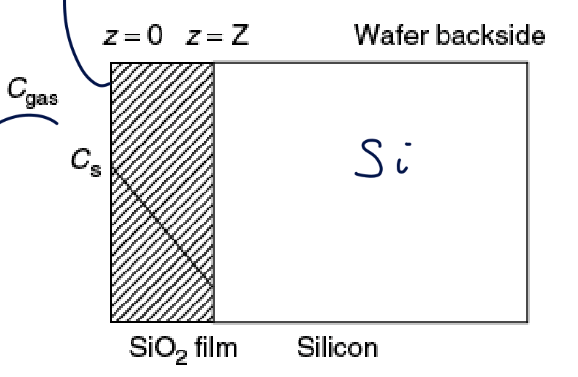
\includegraphics[width=0.95\linewidth]{growth_of_oxide.png}
    \caption{Growth of oxide}
    \label{fig:oxide-growth-label}
\end{wrapfigure}

Silicium will naturally form an oxide and will grow a thin layer of it. This process is only for $Si$ and not present in other type of semi-conductor such a $GaAs$, $Ge$, ... This oxide can be used as :

\begin{itemize}
    \item Implant, diffusion mask
    \item Surface passivation
    \item Isolation between transistors
    \item Key component of MOS structures
    \item Dielectric for multilevel interconnect
    \item Cleaning
\end{itemize}

As shown on the figure, the concentration of oxygen will reduce the further we go towards the right which explains the slowing down of the process. This will create a \textbf{consumption} effect where the oxide will grow upwards and backwards. 1 mole of $SiO_2$ is taking up more volume than 1 mole of $Si$. If we grow $d$ thickness of oxide, we will have $0.46d$ of Si consumed.

\begin{itemize}
    \item $Si$ : $2\cdot 10^{-23} cm^3$
    \item $SiO_2$ : $4.4\cdot 10^{-23} cm^3$ so about $2.2$ times bigger than $Si$. Expansion will go both ways.
\end{itemize}

\subsection{Wet and dry}

\begin{align}
    \text{Dry: }& Si + O_2 \rightarrow SiO_2 & \text{Wet: }& Si + 2H_2O \rightarrow SiO_2 + 2H_2
\end{align}

In \textbf{dry and wet} oxide growth, a higher temperature will lead to thicker oxide growth. This growth will decrease as times grows since the concentration of oxygen diminish. The growth rate is faster in \textit{wet oxide} but it has lower quality which makes it easier to etch.

Since temperature plays a major role, we will have \textbf{oxidation furnace} where our wafers loaded on quartz boat will slowly roll into the furnace which has multiple temperature zone for better control.

\begin{itemize}
    \item Dry: slower growth rate, better quality, better breakdown voltage ($5-10MV/cm$) better suited for gate using \gls{ald}.
    \item Wet: faster growth rate, lower quality, good for masking and interconnect dielectric.
\end{itemize}

For a growth of $0.5\mu m$ of oxide at $1200 C^\circ$ it takes around 6 hours for dry and around 1 hour for wet oxidation.


\subsection{\gls{locos}}

It is a process used for \textit{isolation between transistor}. We can simply use \textit{patterned oxide} as the steps (the transistor) are too high and we can't do spin coating or metallisation. Reduction of topography by about $56\%$. 

To do some masking of oxide we can use $Si_3N_4$ which grows slower than $Si$. But this technique will introduce some stress due to the thermal expansion of nitrite being much higher than of $Si$. We will add between the substrate and the nitrite a small oxide called \textit{pad-oxide} ($SiO_2$) as a stress release layer.

\begin{enumerate}
    \item We first add the pad-oxide of $20-30nm$ and then finally the $Si_3N_4$ of around $100-200nm$. 
    \item Wet oxidation to grow the oxide, mechanical stress will cause a \textit{bird's beak} to form.
    \item Remove the nitride with HF-dip to remove the \textit{oxynitrate} and then $H_3PO_3$ (phosphorous acid) to etch nitrite.
    \item Etching of pad-oxide with HF
\end{enumerate}

\subsection{\gls{sti} and \gls{dti}}

\subsubsection{\gls{sti}}

With this method we can avoid the \textit{bird's beak} phenomena. We can do from about $0.25 \mu m$ nodes without much stress. The process flow is as follow : 

\begin{enumerate}
    \item Anisotropic etching of $Si$
    \item Thermal oxidation
    \item Oxidation growth with \gls{cvd} (using \gls{teos} process)
    \item \gls{cmp} of oxide
\end{enumerate}

\subsubsection{\gls{sti} vs. \gls{locos}}

\begin{itemize}
    \item \gls{sti}: The drawn width is almost the effective width. Can place transistor closer increasing the \textit{packing density}. We have a larger drive current for devices with same drawn width. Less topography.
    \item \gls{locos}: The drawn width is bigger than the effective width due to \textit{bird's beak}. To have the same drive current, we need wider transistor which diminish the packing density. Hard to do this process for sub $0.5 \mu m$.
\end{itemize}

\section{Doping}

There is two main process for doping, either Thermal diffusion or Ion implantation. The later one is more modern and we usually go for a mix of those technique.

Doping relies on the idea to put some foreign atoms in the lattice, either group V to negatively charge it (with an extra electron that is free to roam) or with a group III atoms that will create a hole. It will \textit{locally} create a charge difference. Watch out, we can have some \textit{hole recombination} and so have useless mix of group V and III that will just cancels each other.

For doping we can have: 

\begin{enumerate}
    \item Diffusion, using some \textit{diffusion/doping mask}:
    \begin{itemize}
        \item Gas that will bombard the wafer, not straight path so can have border effect
        \item Coating will use a thin film and will also have border effect
    \end{itemize}
    \item Ion implantation, also uses a \textit{diffusion/doping mask} but will be quite different.
\end{enumerate}


\subsection{Diffusion}

It is a common mechanic phenomena where we will have a material that will search for stability and diffuse to reach a stable state.

\subsubsection{Thermal diffusion}

This process happens at high temperature $1000^\circ$ and when the wafer get exposed to dopant material vapor. The \textit{upper limit} is related to the \textbf{solid solubility}. The lower limit is of $10^{13}$. 

One of the advantage of using silicon, is the fact that the doping level will impact the resistance per square making it an easy material to module the resistance of.

\subsubsection{Diffusion Theory}

We have a diffusion \textit{flux} of \textit{impurities} in one dimension. (We are always using x as the vertical direction of diffusion).

\begin{align}
    F &= - D \frac{\partial C(x,t)}{\partial x} & D &= D_0 exp\left( \frac{-E_{\alpha}}{kT} \right)
\end{align}

We have $D$ that is the \textit{diffusion coefficient} in $cm^2/s$. $C$ is the dopant concentration per unit volume. We have $D_0$ that is the diffusion coefficient in $cm^2/s$ at infinite temperature and $E_\alpha$ is the activation energy in $eV$.

At low concentrations of dopant in silicon ($10^{12} - 10^{16} cm^3$) can be seen as constant. With this simplification, we can easily solve the equation, we also see that gold, coper, ... have high diffusion coefficient which is why we tend to avoid such metal in the clean room.

If we do not have a source or sink of the impurity, we know that the \textit{change in impurity concentration with time must equal the local decrease of diffusion flux}:

\begin{align}
    \frac{\partial C}{\partial t} &= - \frac{\partial F}{\partial x} = \frac{\partial}{\partial x} \left( D\frac{\partial C(x,t)}{\partial x} \right) & \frac{\partial C}{\partial t} &=  D\frac{\partial^2 C(x,t)}{\partial x^2} \text{ if D cst}
\end{align}

There are 2 methods of diffusion:

\begin{enumerate}
    \item \underline{Constant-surface-concentration:} using vapor, we have a constant concentration of dopants at the surface.
    \item \underline{Constant-total-dopant:} thin layer, we have constant amount of impurity at the surface.
\end{enumerate}

\subsubsection{Constant-surface-concentration}

\begin{align}
    \text{Init: } C(x,0) &= 0 & C(0,t) &= Cs & C(\infty, t) &=0\\
    C(x,t) &= C_S erfc\left( \frac{x}{2\sqrt{Dt}} \right) & erfc(z) &= 1-erf(z) & erf(z)&=\frac{2}{\sqrt{\pi}}\int_0^\pi e^{-y^2} dy
\end{align}

We have $\sqrt{Dt}$ that is called the \textit{diffusion length} in $cm$. The total number of dopant atoms per unit area that has diffused into the semiconductor is given by:

\begin{equation}
    Q(t) = \int_{0}^\infty C(x,t) dx = \frac{2}{\sqrt{\pi}} C_s \sqrt{Dt} \approx 1.13 C_s \sqrt{Dt}
\end{equation}

\subsubsection{Constant-total-dopant}

\begin{align}
    C(x,0) &= 0 & \int_0^\infty C(x,t) dx &= \phi & C(\infty, t) &= 0\\
     & & C(x,t) &= \frac{\phi}{\sqrt{\pi D t}} exp \left( - \frac{x^2}{4 D t} \right)
\end{align}

Where $\phi$ is the \textit{total amount of dopant} per unit area. So the surface concentration ($x=0$) is $\phi / \sqrt{\pi Dt}$.

We usually use those two methods and we call this a \textit{two step diffusion process}. a pre-deposition diffused layer is first formed using constant-surface-concentration condition. Then a drive-in (or redistribution) diffusion is used using constant-total-dopant condition.

For most practical cases the diffusion length for the pre-deposition stage is much smaller than the diffusion length of the drive-in diffusion. This allows to make deep junctions, e.g. for wells for CMOS.

\subsubsection{Advanced Diffusion Theory}

We are oversimplifying the problem which will gives us incorrect values when compared with reality. Moreover, the atoms vibrate and there is a non-zero chance that a silicon atom moves from its lattice site which will leave a vacancy.

Dopants diffuse in combination with silicon interstitials or vacancies and the diffusion coefficient is therefore strongly influenced by the concentration of interstitials or vacancies.

\subsubsection{High Doping Concentration Diffusion}

Here, our simple theory doesn't hold anymore. The diffusion profile is different. Moreover, the diffusion of phosphorous at high concentration is \textit{anomalous}. We often notice a \textit{kink} on the doping profile. Then we have a deep tail region that extends further in the doping region.

The anomalous diffusion behavior has been explained by the dissociation of the phosphorus-vacancy pair (P+V2-) into P+, V- and an electron. The singly charged acceptor vacancies (V-) enhance the diffusivity in the tail region (by a factor of 100 at $1000^\circ$). So it is good for creating deep n-type junction. Arsenic is preferred over phosphorous.

\begin{table}[H]
    \centering
    \renewcommand{\arraystretch}{1.3}
    \begin{tabular}{|l|c|c|c|}
        \hline
        \textbf{Dopant level} & \textbf{Designation} & \textbf{Dopant concentration} (cm$^{-3}$) & \textbf{Resistivity n/p} (ohm-cm) \\
        \hline
        Very lightly doped & n$^{--}$, p$^{--}$ & $<$10$^{14}$ & $>$100/$>$30 \\
        Lightly doped & n$^{-}$, p$^{-}$ & 10$^{14}$–10$^{16}$ & 1–100/0.3–30 \\
        Moderately doped & n, p & 10$^{16}$–10$^{18}$ & 0.03–1/0.02–0.3 \\
        Highly doped & n$^{+}$, p$^{+}$ & 10$^{18}$–10$^{19}$ & 0.01–0.03/0.005–0.02 \\
        Very highly doped & n$^{++}$, p$^{++}$ & 10$^{19}$ & 0.001$<$0.01/0.005 \\
        \hline
    \end{tabular}
    \caption{Doping levels, designations, concentrations, and resistivities.}
    \label{tab:doping_levels}
\end{table}

Here, we are always talking in $\Omega / cm$ resistance that relates to the sheet resistance.

For diffusion we can either have diffusion through substitutional or interstial diffusion.

\subsubsection{Using $SiO_2$ for masking}

The diffusion of $B,P,As$ in $SiO_2$ is at least one order of magnitude lower than in $Si$. There exists some table that indicates the thickness of the oxide for the diffusion of a given material at a given temperature during a definite amount of time.

By mixing impurities, we can slowly diffuse some up to a deep depth and then diffuse another type. They will cancel each other out which will create some junction and deeper junction.

\begin{figure}[H]
    \centering
    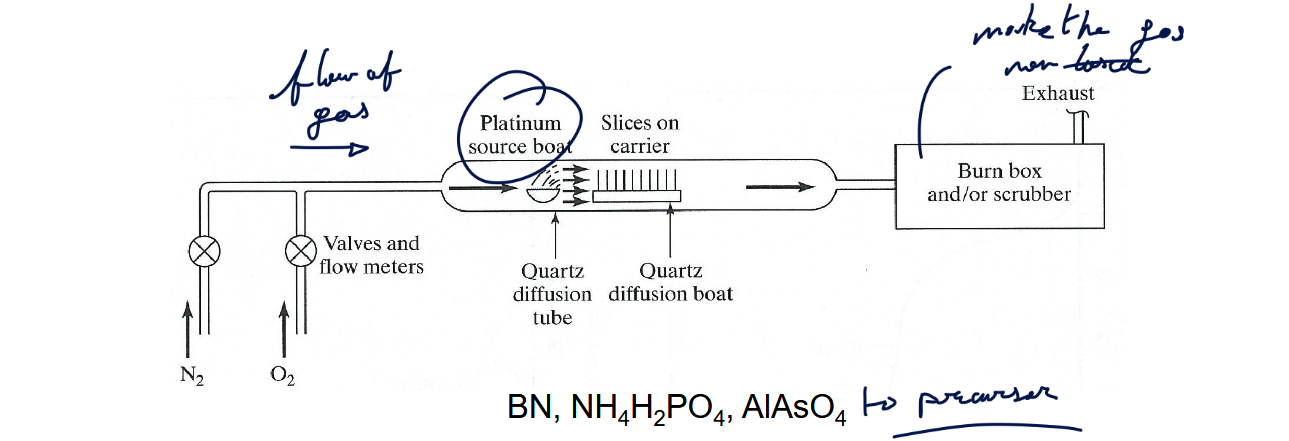
\includegraphics[width=0.75\linewidth]{solid_dopant_sources.png}
    \caption{Solid Dopant Sources}
    \label{fig:SDS-label}
\end{figure}

The boat we are using has some Boron nitride wafers between 2 substrate wafers to diffuse it. 

There is also a version that uses liquid dopant sources which is similar to the solid dopant one except the $N_2$  will be bubbling in the bubbler. We can also have the same with gas using some dopant gas. We have to add some scrubber system to trap all of the gases.

\section{Ion implantation: deposition, drive-in and RTA}

\begin{figure}[H]
    \centering
    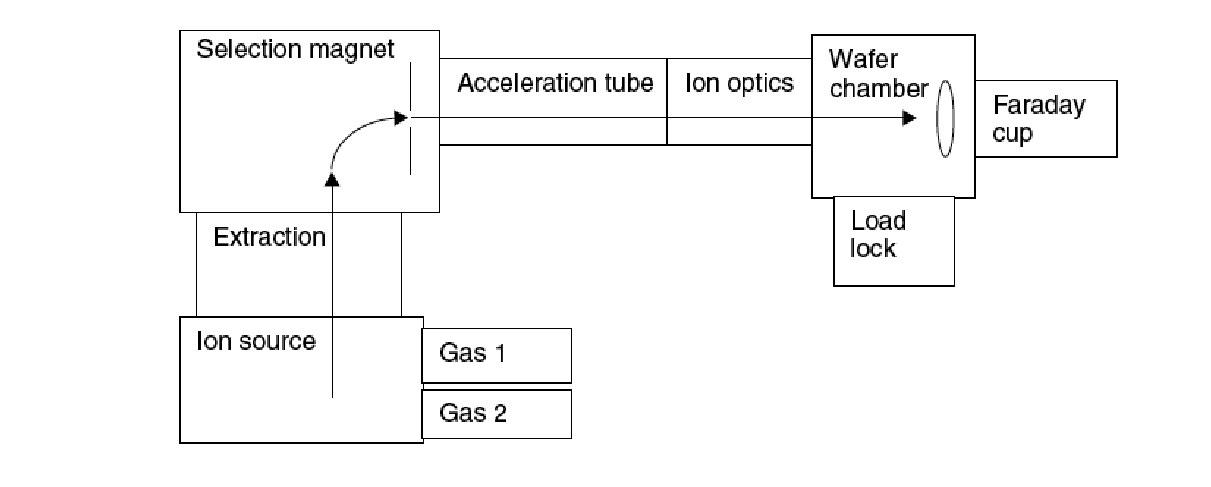
\includegraphics[width=0.75\linewidth]{ion_implantation.png}
    \caption{Basic elements of an ion-implanter}
    \label{fig:ion-implanter-label}
\end{figure}

\begin{enumerate}
    \item \underline{\textbf{Ion source:}} it works at high voltage $25 kV$ and creates a plasma with the desired impurity.
    \item \underline{\textbf{Mass spectrometer:}} it will selects which ion we want in this right angle bend.
    \item \underline{\textbf{High voltage accelerator column:}} to make it faster we accelerate it with a field of over $5MeV$.
    \item \underline{\textbf{Scanning system:}} to deposit the right amount, we also make it slightly bend so the neutral particles will go straight and not hit the wafer.
    \item \underline{\textbf{Target chamber:}} operated in vacuum conditions and is where the wafer is located in.
\end{enumerate}

Something important to note is the fact that the ions will hit the wafer pretty straight but it will go through a random path in the wafer. This will lead to a gaussian distribution of the particles around a certain depth.

\begin{equation}
    N(x) = N_p exp \left( - \frac{(x-R_p)^2}{2 \Delta R_p^2} \right) \qquad N_p = \frac{\phi}{\sqrt{2 \pi} \Delta R_p}
    \label{eq:ion}
\end{equation}

\subsection{Ion implantation}

So the main idea is "simply" accelerating ions pretty quickly so that they will penetrate inside the wafer up to a few tenths of microns. Of course, masking is used so we can create the desired pattern and not simply bombard the full wafer. We can either use some silicon dioxide or photoresist.

In \ref{eq:ion}, $\phi$ is the \textit{ion dose per unit area} and $R_p$ is the distance to the peak from the surface and is called the \textit{projected range}. $\Delta R_p$ is the \textit{projected straggle} is the distance from the peak where the concentration is reduced by $40\%$ and is usually empirical.

One major advantage and use case of ion implantation is to put some ions below a gate oxide for example. But we damage the lattice by bombarding like this and we require some \textbf{annealing} at $900^\circ$ to repair the damage. If we go even hotter we can do some \textit{drive-in} to diffuse even further the dopant into the silicon.

\subsection{Masking}

Now, how thick should a mask be so all the ions will be trapped inside the mask ? But it is important to note that since it is a Gaussian distribution we will always have a probability that the ions will go inside the substrate. 

Something that is even more annoying is the fact that we will have some ions around a slit that will go under the mask.

\begin{figure}[H]
    \centering
    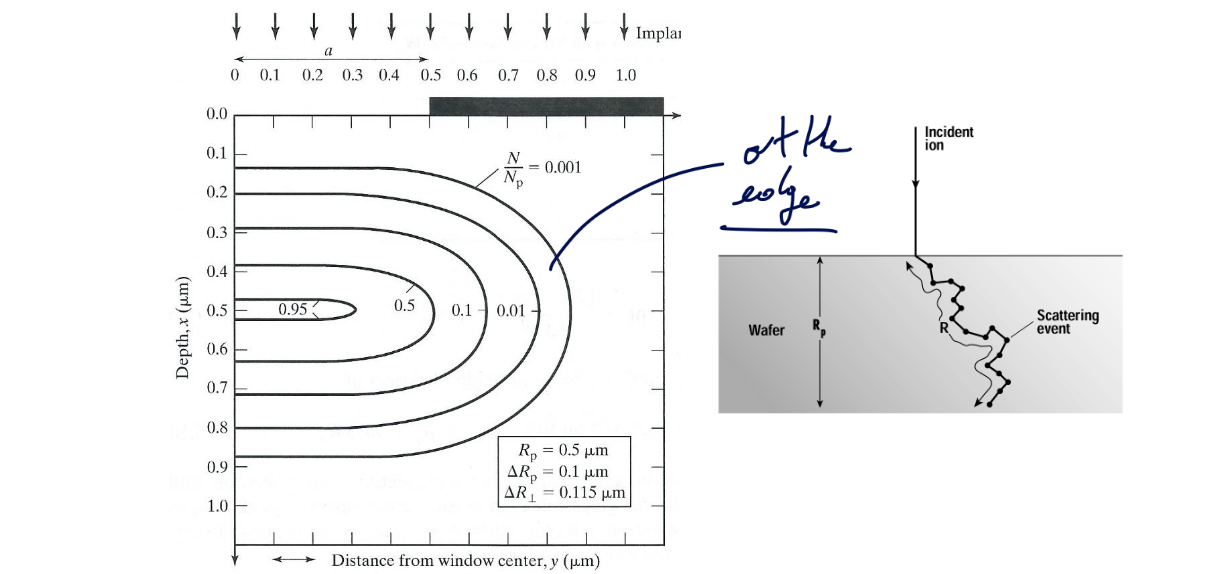
\includegraphics[width=0.75\linewidth]{implanatation.png}
    \caption{Ion Implantation}
    \label{fig:implantation-label}
\end{figure}

We have to realize some empirical experiments to see under which condition a given ions will dope or not the silicon or stop at the silicon dioxide.

\subsection{Annealing}

It is a crucial step after doing some ion implantation where we have to restore the lattice from any damages. But it also allows the dopants to take the correct spot inside the lattice.

As hinted previously, doing this sort of baking at high temperature will lead to some \textit{drive-in} by diffusion and we will have more spread.

\subsubsection{\gls{rta}}

To avoid this diffusion to happen to fast, we can use some lighting bulb to produce a quick and rapid heating of the substrate.

\subsection{Channeling}

One thing that can happen if we have a perfect lattice is the fact that an ion may not bounce and will went through the lattice directly. So instead of having a nice gaussian we will see some odd shapes and multiple peaks.

\subsubsection{Solutions}

We can add a layer of oxide so it will force the ions to bounce around. Or we can tilt the wafer or even grow some \textit{amorphous} Poly-Si.

\subsection{Profile Verification}

After applying a layer, we would like to measure the thickness of an oxide or other things:

\begin{itemize}
    \item \underline{\gls{sims}}
    \item \underline{\gls{srp}:} destructive process since we bombard the surface and measure the amount of ions and neutral particules.
\end{itemize}

There is also electrical measurement where we use two probes and measure the resistivity by applying a current. This will leave some \textit{damage craters} due to the probing. There is another version that uses 4 probes that measures the current and the voltage.


%\chapter{Doping, ion implantations}



\chapter{Etching, wet, dry, plasma, DRIE}

In etching, we distinguish two types:

\begin{itemize}
    \item Isotropic: the etching goes in every direction and etches pretty equally
    \begin{itemize}
        \item Plasma, Wet (mostly), \gls{rie}
    \end{itemize}
    \item Anisotropic: the etching prefers one orientation of the lattice
    \begin{itemize}
        \item Plasma, \gls{rie}, Ion milling, \gls{drie}, KOH wet
    \end{itemize}
\end{itemize}


\section{Wet Etching}

\subsection{Isotropic}

To keep a constant gradient locally, we have to replace all the time the solution that's why we overflow the bath by adding continuously new etchant and uses a stirer.

Because of the way wet etching works, we will have \textbf{undercut area} that we also call \textit{etch bias} and can be an issue for features that are too close to each other. Below $3 \mu m$ we will prefer dry etching.

To stop precisely and quickly the reaction, we use a a trap at the bottom of the bath to quickly dump the etchant and we spray the wafer with solution to stop quickly and precisely the process.

\begin{table}[hbt]
\centering
\renewcommand{\arraystretch}{1.2}
\begin{tabular}{|l|l|}
\hline
\textbf{Material} & \textbf{Etchant} \\
\hline
SiO$_2$ & $NH_4F:HF \ (7:1)$ BHF, $35^\circ C$ \\
\hline
SiO$_2$ & ${NH_4F:CH_3COOH:C_2H_6O_2:H_2O} \ (14:32:4:50)$ \\
\hline
poly-Si & ${HF:HNO_3:H_2O} \ (6:10:40)$ \\
\hline
Al & ${H_3PO_4:HNO_3:H_2O} \ (80:4:16)$, \\
   & water can be changed to acetic acid \\
\hline
Mo & ${H_3PO_4:HNO_3:H_2O} \ (80:4:16)$ \\
\hline
W, TiW & ${H_2O_2:H_2O} \ (1:1)$ \\
\hline
Cr & ${Ce(NH_4)NO_3:HNO_3:H_2O} \ (1:1:1)$ \\
\hline
Cu & ${HNO_3:H_2O} \ (1:1)$ \\
\hline
Ni & ${HNO_3:CH_3COOH:H_2SO_4} \ (5:5:2)$ \\
\hline
Ti & ${HF:H_2O_2}$ \\
\hline
Au & ${KI:I_2:H_2O}$; ${KCN:H_2O}$ \\
\hline
\end{tabular}
\caption{Etchants for various materials}
\end{table}

We can also use other etchant or use some HF that is often used for $SiO_2$. But HF is pretty dangerous to handle as a spill on your skin doesn't burn or causes pain immediately, it will slowly penetrate the body until it attacks the bone.

\subsection{Anisotropic}

We also have some anisotropic wet etchant where we will have various effect depending on the lattice orientation (using the notation as seen previously):

\begin{figure}[H]
    \centering
    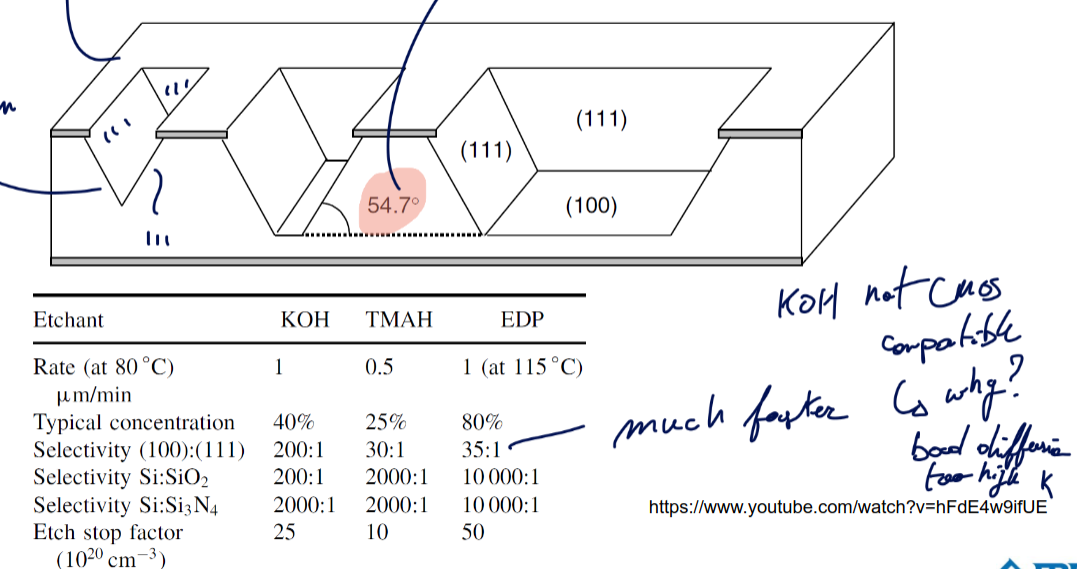
\includegraphics[width=0.75\linewidth]{ansitropic_wet.png}
    \caption{Anisotropic wet etching}
    \label{fig:enter-label}
\end{figure}

\section{Dry Etching}

This process comes in many flavors but they are all a combination of some excitation energy and pressure where we either have high energy-low pressure or low energy-high pressure. We use mechanical and chemical aswell to better control the process.

\begin{itemize}
    \item Physical: we bombard the wafer with some \textit{positive ions} and we strike the substrate with high kinetic energy.
    \item Chemical: we can either use neutral or ionized species to react with the surface to create some \textit{volatile product}. This process is often \textit{isotropic}.
\end{itemize}

\subsection{Plasma Etching}

Plasma is a \textit{fully or partially} ionized gas containing an equal amount of positives and negatives charges but has different number of unionized molecules. We then need a strong enough electrical field to ionize the gas.

The goal of plasma etching is to produce some chemically reactive species from a relative inert gas. Then we make this gas react with the specific material we want to etch and the product should be pretty volatile to be easily removed. We need high speed and high chemical reactions between neutrals and the substrate materials. We use a \textit{carrier} gas producing some ions and reactive neutrals. This reactive neutrals attack the sidewall and the normal surface. BUT, the positive ions will \textbf{only} attack the normal surface. So we will first go in the vertical direction.

We have around $10^{15} cm^{-3}$ and $10^8-10^{12} cm^{-3}$. After hitting the surface, we may have the volatile particles to react against the wall of the chamber which is really problematic. But washing is not always the solution as it can disrupt the precise setting for the reaction to happen at an optimal point.

To have some idea about the type of gases we can use look at the various tables chapter 5 page 30-32.

\subsection{Ion milling - \gls{drie}}

Ion milling is a sort of \textit{sputter etching} where the wafer is coupled to a voltage source. It also uses some plasma gas but the added voltage to the wafer add some acceleration to the positive ions.

\begin{figure}[H]
    \centering
    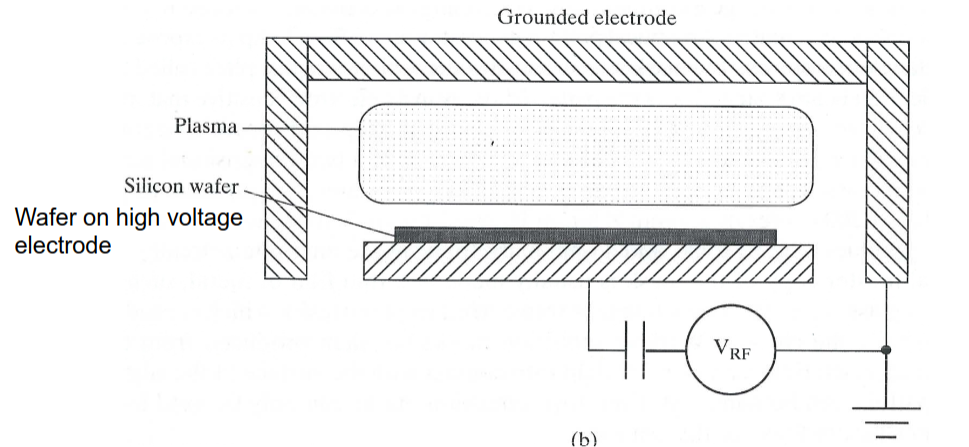
\includegraphics[width=0.75\linewidth]{rie_setup.png}
    \caption{\gls{rie} setup}
    \label{fig:rie-setup-label}
\end{figure}

\subsection{\gls{rie}}

It is a combination of plasma etching and sputter etching/ion milling since we use some plasma and accelerate it towards the susbtrate. Again we use a chemical and mechanical process. 

The setup is pretty similar as depicted in \ref{fig:rie-setup-label}, we use the asymmetry between electrodes to create a self-bias to accelerate the ions towards the substrate. We can also add additional electrodes to create a DC electric field.

It is a combination of chemical and sputtering:

\begin{enumerate}
    \item Chemical:
    \begin{itemize}
        \item Thermalized neutral radicals that will form volatile products.
        \item Isotropic
        \item little electrical damage
    \end{itemize}
    \item Sputtering:
    \begin{itemize}
        \item Ion energy will mechanically ejects substrate material
        \item Anisotropic
        \item Purely physical and pretty directional, low pressure so longgg \gls{mfp}
        \item Low etch rate
    \end{itemize}
\end{enumerate}

\begin{figure}[H]
    \centering
    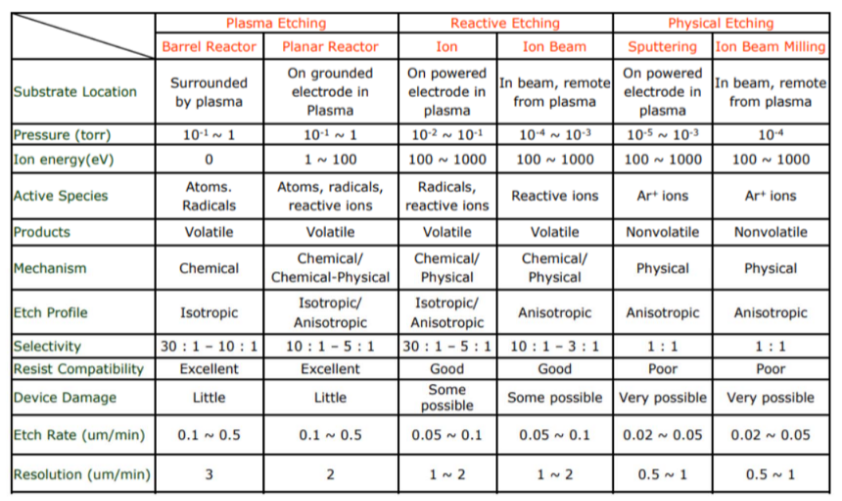
\includegraphics[width=0.75\linewidth]{rie_etching_possibilities.png}
    \caption{\gls{rie} etching possibilities}
    \label{fig:enter-label}
\end{figure}

There is two categories of \gls{rie} etching:

\begin{enumerate}
    \item \underline{Ion-Induced \gls{rie}:} reaction controlled etching with typically $Cl_2/Si$
    \begin{itemize}
        \item When subststrate is not spontaneously etched away
        \item Ions modify the surface reactions in one way or another. Make the radicals to react with the substrate.
    \end{itemize}
    \item \underline{Ion-Inhibitor \gls{rie}:} desorption-controlled etching with typically $F/Si, Cl_2/Al$.
    \begin{itemize}
        \item Substrate is etched spontaneously so we need an inhibiting layers to achieve directionality.
        \item The bottom of the trench is exposed to ion bombardment.
    \end{itemize}
\end{enumerate}

\subsubsection{Fluorine-Based Plasma - Anisotropic Si etching}

Due to the isotropic nature of the chemical reaction, we have to use some inhibitor layer composed of Silicium, Fluor and oxygen. This is some ion-inhibitor process and the oxygen covers the silicon surface with silicon oxide. The issue is that the SF5+ will etch the layer making it possible for the F* radicals to etch the silicon substrate.

\subsubsection{Chlorine-Based Plasma - Thin-film Al Dry etching}

Aluminum is spontaneously etched by $Cl_2$ but there is a native aluminum oxide layer. We have to use some ion bombardment because it is essential for aluminum.

\subsubsection{Chlorine-Based Plasma - Poly-Si Dry etching}

We use som ion-induced \gls{rie} with gases like $Cl_2, HBr, O_2$.

\subsubsection{Ion Milling Etching: thin film platinum etching}

We use some $Ar$ gas and the platinum has been \textit{physically} etched by argon plasma. We can witness some sort of fence because the platinum may redeposit on the sidewall creating some fences.

\subsubsection{Inductively coupled Plasma \gls{rie}}

Here we use some \gls{ccp} to etch the silicon and other material slowly. \gls{icp} \gls{rie} generates the plasma through a RF powered magnetic field which allows us to create some very high plasma density.

\begin{figure}[H]
    \centering
    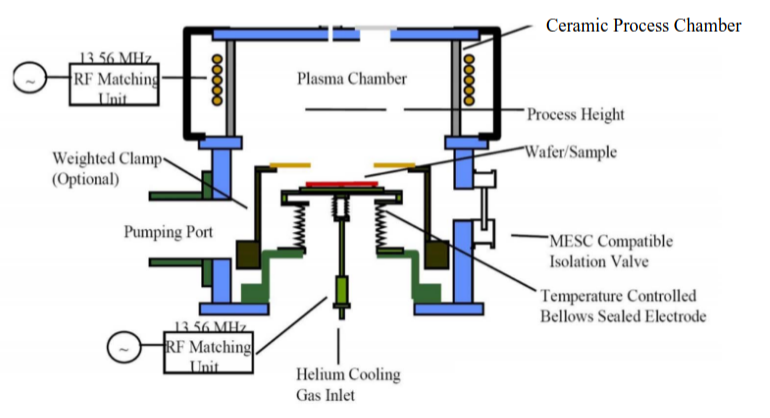
\includegraphics[width=0.75\linewidth]{Setup_plasma_rie.png}
    \caption{Plasma coupld \gls{rie}}
    \label{fig:enter-label}
\end{figure}

\subsection{\gls{drie}}

We also use some \gls{drie} or Bosh process that allows us to draw some pretty precise features with a high-aspect ratio (20-50), it is a cyclic process where we alternate between etching and depositing. We etch using some $SF_6$ and deposit some polymer layer of $C_4F_8$. We can etch over $10 \mu m/min$ and go through the whole wafer. We pulse but it will still eat a bit of the sidewall. It is pretty good for MEMS devices.

\subsubsection{Etch Lag}

A bigger opening will etch more vertically compared to a shallower one with the same amount of cycles.

\subsection{Comparing Dry etching}

\begin{table}[H]
\centering
\begin{tabular}{|l|l|}
\hline
\textbf{Etching Mode} & \textbf{Pressure (Torr)} \\
\hline
Ion Milling & $10^{-4}$ -- $10^{-3}$ \\
Reactive Ion Etching/Ion Milling & $10^{-3}$ -- $10^{-1}$ \\
Plasma Etching & $10^{-1}$ -- $5$ \\
\hline
\end{tabular}
\caption{Etching Pressure Ranges}
\end{table}


\chapter{Interconnects, Al, Cu, CMP}

Interconnect is a crucial part of any IC's as they connect the various transistors among each other and to connect the IC with other components.

We first considered Aluminum for interconnect as it is cheap, compatible with Si technology, it adheres well to SiO2. One major flaw is the low melting point of 577 c. Copper was for a long time avoided as it diffuses really fast in Si and SiO2 and adheres not really well to SiO2.

\section{Aluminum as interconnect}

\subsection{Spiking and pitting}

Silicon will naturally diffuses non-uniformly into Aluminum creating \textbf{spiking}, this Silicon that diffuses will leave some space that the Aluminum will "\textit{fall}" into it due those pits.

Those pits could break some junction inside of a transistor.

\subsubsection{Solution}

Add some Silicon to the Aluminum or during the PVD step. We can also add some barrier metrial as Titanium-Tungsten.

\begin{figure}[H]
    \centering
    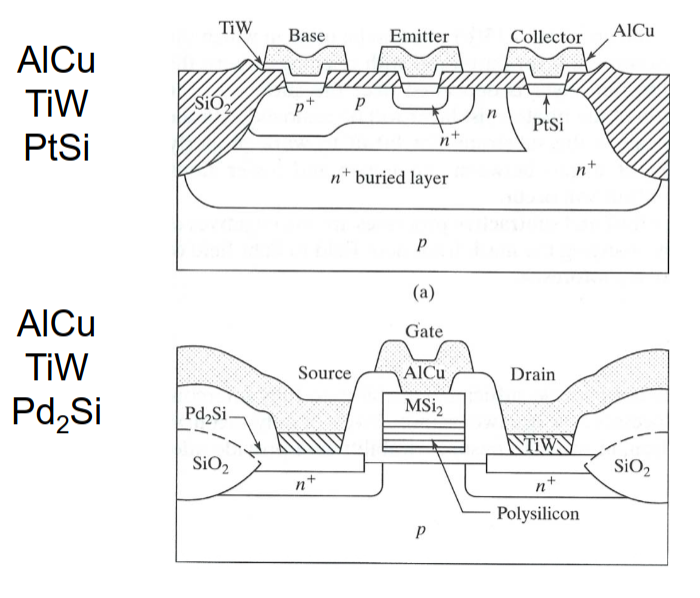
\includegraphics[width=0.5\linewidth]{Solution_tiw.png}
    \caption{Barrier solution to TiW}
    \label{fig:TiW-label}
\end{figure}

\subsubsection{Silicides}

Silicium can react with various metal which have various resistivity and can appear at different conditions. Those properties can be used to make some metal to react with the wafer, the rest of the metal that didn't react with the silicium.

\subsection{Electromigration}

If we make the interconnect too thin we can witness electrons carrying away some chunk of metal. Also good to remember that the flow of current is opposite to the flow of electrons. 

\subsubsection{Solution}

We can add Cu to Al, 95 \% Aluminum, 4\% copper and 1\% Silicon. Or the simple solution is to use some Cu.

\subsection{Multilevel Metal Problem}

We will have non planar structure in our wafer with all those layers and structures we form. We will have some \textbf{via-depth} problem.

\subsubsection{Solution}

This is why we usually make the contact wider and wider contacts as the stack increase. We can also slightly shift the stacking to avoid alignment issues.

We also have developed techniques to make the structure more planar by filling up via with tungsten through \gls{cvd} and we also deposit some Aluminum using \gls{pvd}. The filling of tungsten is a \textit{selective deposition} as seen with the reaction:

\begin{equation}
    2 WF_6 (g) + 3 Si (s) \longrightarrow 2 W (s) + 3SiF_4 (g)
\end{equation}

\begin{figure}[H]
    \centering
    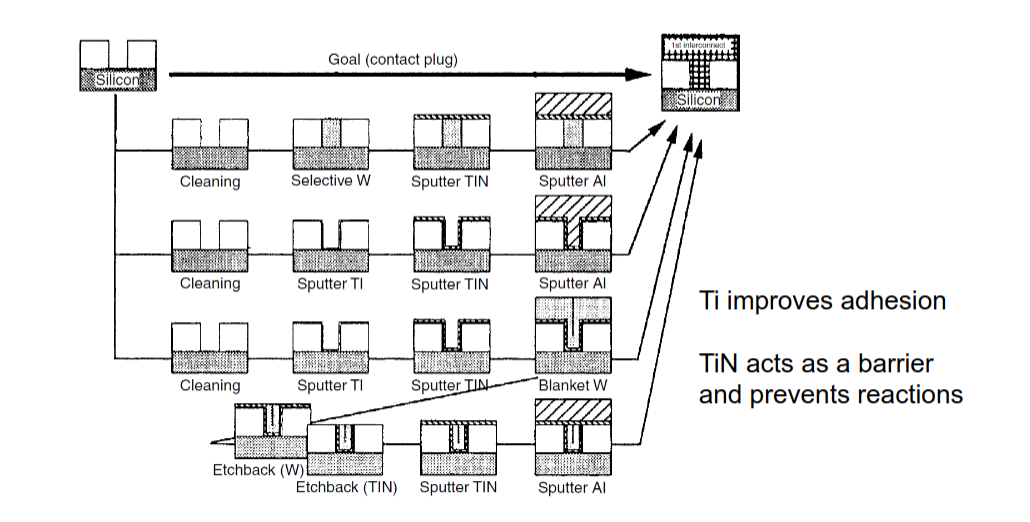
\includegraphics[width=0.75\linewidth]{contact.png}
    \caption{Several ways  to create interlayer contacts}
    \label{fig:enter-label}
\end{figure}

\subsection{\gls{cmp}}

\subsubsection{Planirize the surface}

A common used techniques is to use oxide-\gls{cmp} to planirize the surface after applying some contacts. Then we can build on top of a flat and clean surface.

Another way is to use some \gls{cmp} that uses a \textbf{chemo-mechanical polish}. It can be used to:

\begin{enumerate}
    \item Smoothing
    \item Planarization: ideal after applying some interconnect
    \item Damascene: a commonly used techniques in Cu interconnet and allows to draw some precise features
\end{enumerate}

\subsubsection{\gls{cmp} principle}

\begin{figure}[H]
    \centering
    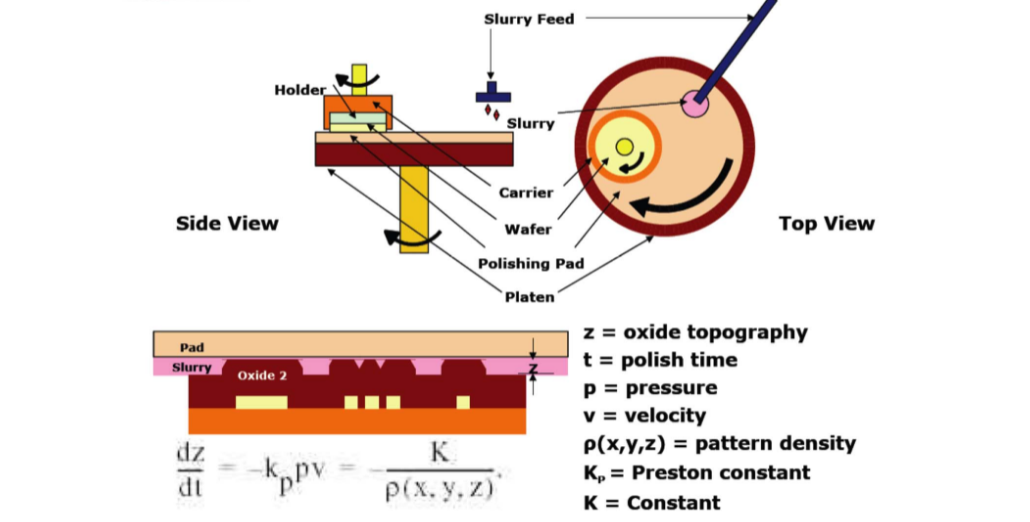
\includegraphics[width=0.75\linewidth]{cmp_lucent.png}
    \caption{\gls{cmp} principle}
    \label{fig:enter-label}
\end{figure}

It is a pretty staight-forward process, we can also have some \textit{multiwafer} machinery that allows us to process multiple wafer in parallel.

This process is not perfect and can smooth out \textit{local} planarity but it will distribute it \textit{globally} resulting to global non-planarity which is not really the desired effect.

\subsubsection{Solution to reach global planarity}

\begin{figure}[H]
    \centering
    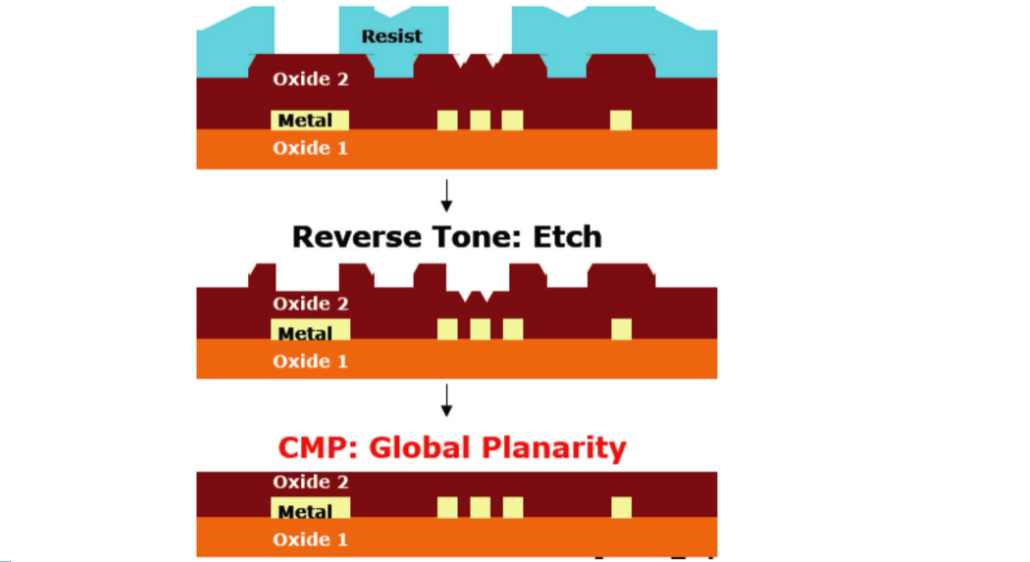
\includegraphics[width=0.65\linewidth]{global_planarity.png}
    \caption{Global planarity}
    \label{fig:enter-label}
\end{figure}

Another solution would be to add dummy oxide which will make the \gls{cmp} smoother. This dummy oxide can sometimes be seen in finished products.

\subsection{Copper IC}

The main reason to push for copper interconnect, is to further reduce the delay time as we scale down.

\begin{figure}[H]
    \centering
    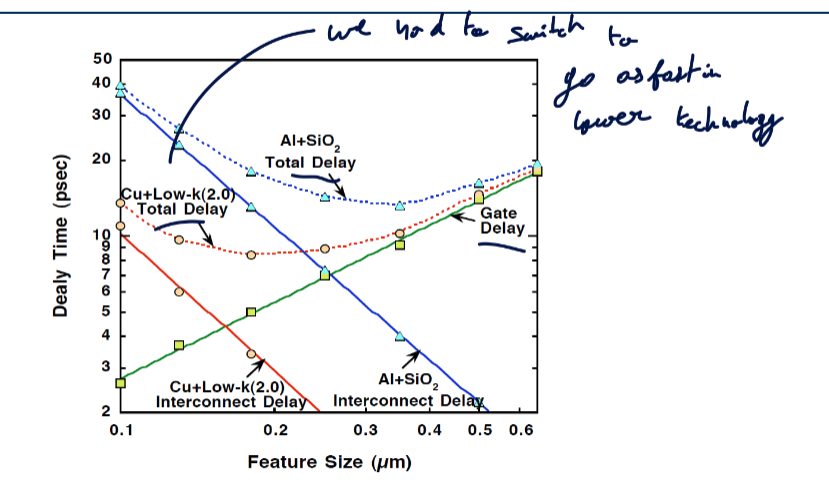
\includegraphics[width=0.5\linewidth]{copper_ic.png}
    \caption{Copper interconnect}
    \label{fig:enter-label}
\end{figure}

It also has some better resistance against failure but it doesn't adhere well to dielectric, it diffuses with the dielectric. It is compatible with tungsten plug (good point) but the copper just contaminate the chip and the equipment, ...

So to avoid this, we will use some \textit{seed layer} that behaves as a sort of protective layer. The damascene process is extensively used to produce some pretty flat result.

\begin{figure}[H]
    \centering
    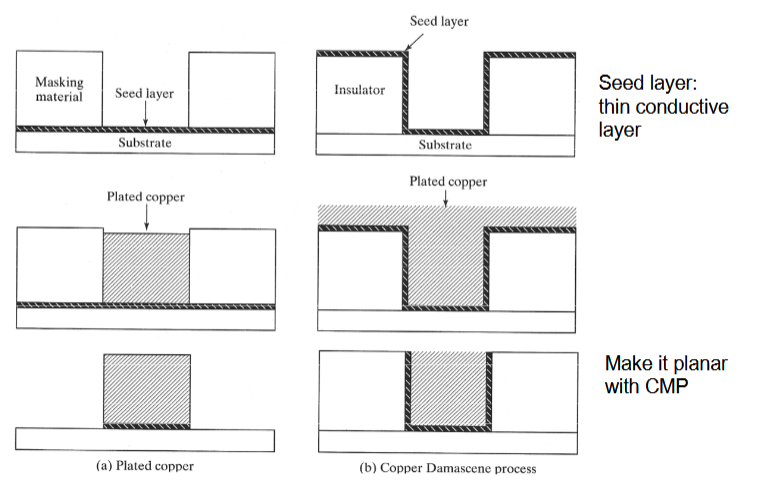
\includegraphics[width=0.5\linewidth]{electroplating.png}
    \caption{Copper, electroplating}
    \label{fig:enter-label}
\end{figure}

\subsubsection{Damascene process}

\begin{wrapfigure}{r}{0.24\textwidth}
    \centering
    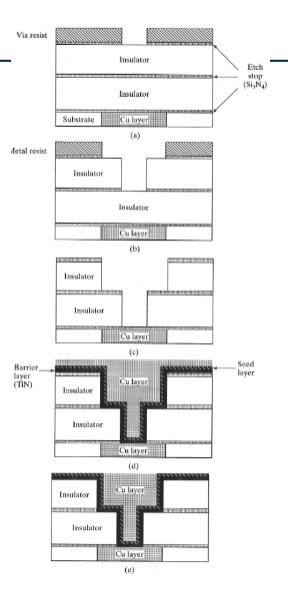
\includegraphics[width=0.9\linewidth]{dual_damascene.png}
    \caption{Dual damascene}
    \label{fig:enter-label}
\end{wrapfigure}

The idea behind this process, is to simply add this protective layer (through \gls{ald}), deposit the copper and polish using \gls{cmp}.

The dual damascene process is extensively used in vias and interconnect traces as it can make some thicker top traces

It is the de facto standard in CMOS processing. This allows to create complex stack with many many layers.

If we are using the simple platting of copper, we can use some lift-off process which makes removing the excedant of copper quite easy. Employed especially for \ce{Au} and \ce{Pt}.


\chapter{IC Processing overview}

\section{CMOS}

\begin{figure}[H]
    \centering
    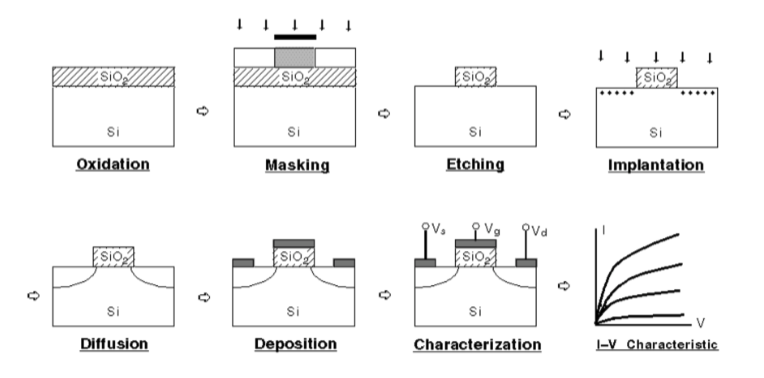
\includegraphics[width=0.5\linewidth]{simplified_CMOS.png}
    \caption{The simplified CMOS processing}
    \label{fig:enter-label}
\end{figure}

In the beginning, we used a lot of \ce{Al} gate to control the gate which was a sensible choice given the easy of connection and we just have some thermal diffusion. But the biggest issue and limitation was the fact that it was not a \textbf{self-aligned process}. Meaning that engineer had to take margin when doing the gate creating some unnecessary overlap which amplified the junction capacitance further reducing the speed. On top of this, after applying \ce{Al} we couldn't do a lot of other processes that works at higher temperature !

In Aluminium process, we first dope through some high temperature step then we need to align the gate on top of the source and drain.

But now, in poly-gate, we can whistand higher temperature and here we use the poly gate as the mask for the source and drain region. \textbf{The gate comes first, forcing the source and drain to be at the right place}.

\subsection{Self-alignment}

\begin{figure}[H]
    \centering
    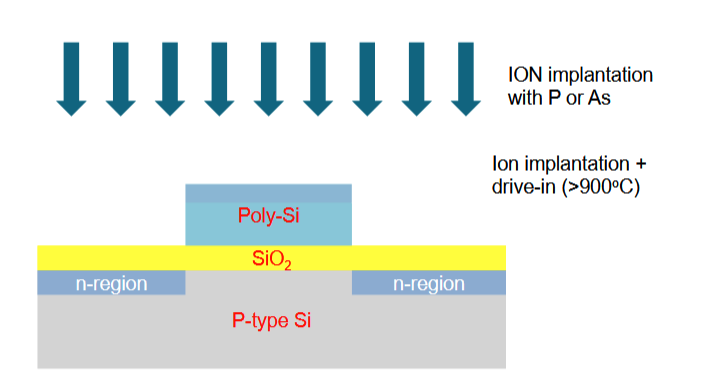
\includegraphics[width=0.5\linewidth]{self_alignment_poly.png}
    \caption{Self-alignment polygate}
    \label{fig:enter-label}
\end{figure}



\subsection{Basic flow}

We first start "drawing" the poly-silicon gate using a mask. We do for the NMOS and PMOS at the same time. Once it is done, we remove the photoresist, do some Boron implantation for NMOS. We implant some Arsenic with low-energy (so we don't put too many) which acts like a channel stop, to avoid any charges during operation to flow from a NMOS to PMOS.

\begin{figure}[H]
    \centering
    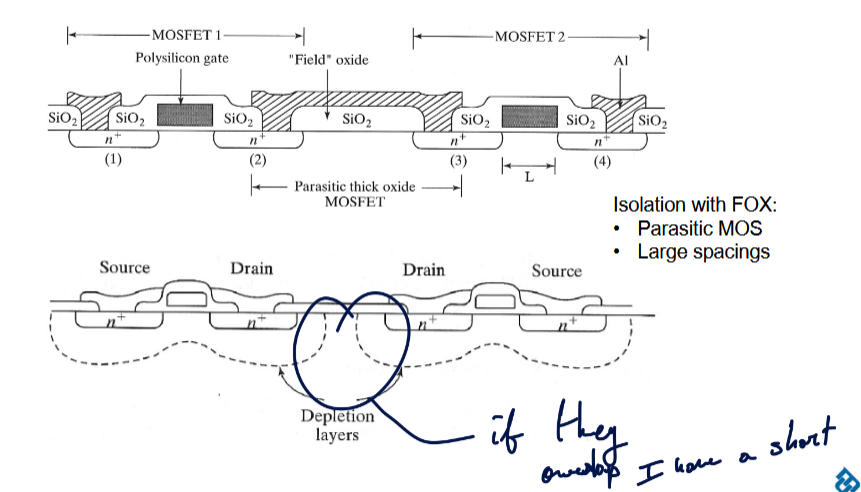
\includegraphics[width=0.5\linewidth]{parasitic_NMOS.png}
    \caption{Parasitic NMOS thick}
    \label{fig:enter-label}
\end{figure}

In this process step, we can find back the \gls{locos} process and see the appearance of those bird's beak. Then we apply remove the Nitride to implant some Boron for the PMOS.

Once we have the desired region for the channel, we can add the polysilicon and \textbf{then} the actual doping with some high dose boron for PMOS and high dose phosphorus for NMOS. We just have to invert the mask from the previous step. It is self-aligning since the implantation will slightly bend around the gate which will create a controlled channel capacitance.

Finally, we can do some \gls{cvd} deposition of the contact holes and finish it with some nice metallization and etching. And voilà ! we have a CMOS. Ofc, it is not flat and nice as depicted in schematics. It is quite chaotic and uneven.

\subsubsection{Latch-up}

One big enemy: Latch-up ! Typically there is some undesired bipolar junction that forms a \textit{thyristor}. So for this we usually use some \gls{epi} and \gls{sti} to ensure no such behavior can occur.

\begin{figure}[H]
    \centering
    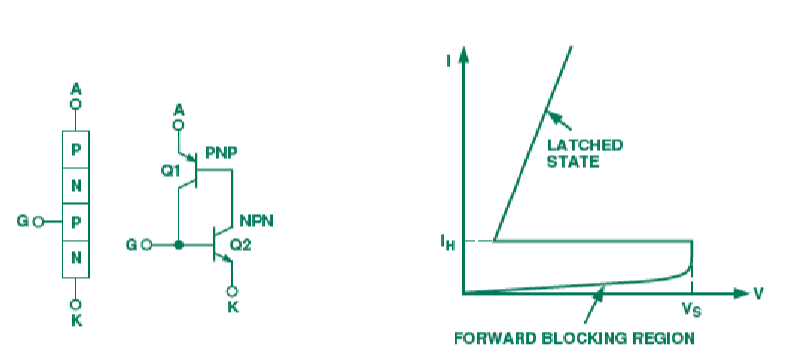
\includegraphics[width=0.5\linewidth]{thyristor_operation.png}
    \caption{Thyristor and its operation}
    \label{fig:enter-label}
\end{figure}

\begin{figure}[H]
    \centering
    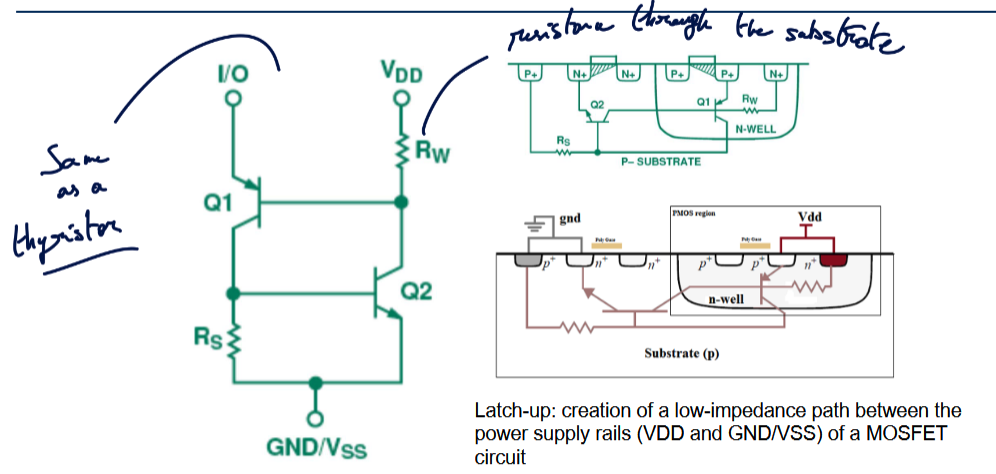
\includegraphics[width=0.5\linewidth]{latchup.png}
    \caption{Latch-up}
    \label{fig:enter-label}
\end{figure}

So this is why we love \gls{sti} in this case !

\subsection{Advanced CMOS process}

We use a base substrate p where we grow some \gls{epi} on top, we then depose some \ce{SiO2} with a buffer layer made of nitride. We use some plasma etching to create trenches using the inverse of the active area mask.

\begin{figure}[H]
    \centering
    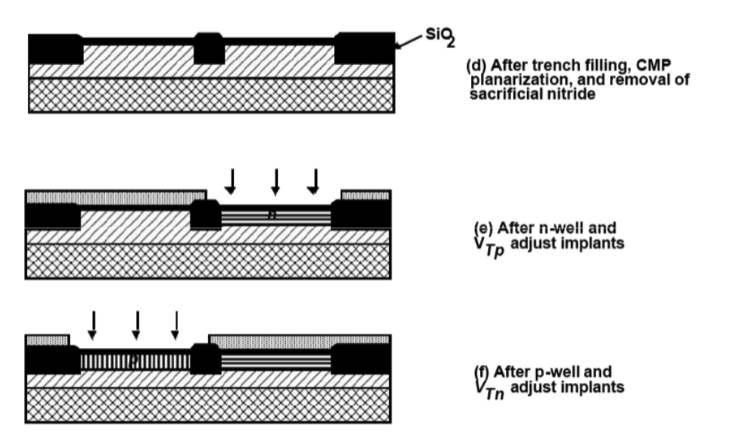
\includegraphics[width=0.5\linewidth]{advanced_cmos.png}
    \caption{Advanced CMOS process}
    \label{fig:enter-label}
\end{figure}

But this isn't always enough and sometimes, we need to do some \gls{ldd} to avoid \textit{hot electron} effect. This effect can sometimes change the actual doping which can then destroy the junction and make MOS not work at all !

\subsubsection{Hot carrier effect}

It happens when a strong EM field is applied and when an electron has enough \textit{kinetic energy} to break lattice bonds and hence create another electron-hole pair. They have an energy over $kT$. This will increase the current in the channel but the holes will be absorbed by the substrate creating a little current that can be monitored. This creates a sort of BJT.

This is why we often add some spacer to help with this effect.

\subsection{Salicide}

It allows a better current flow synonym of more freedom in the layout !

\begin{figure}[H]
    \centering
    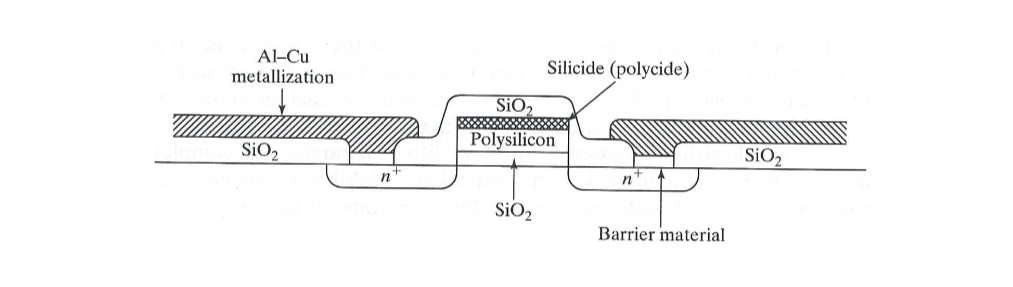
\includegraphics[width=0.5\linewidth]{polycide_salicide.png}
    \caption{Polycide - Salicide}
    \label{fig:enter-label}
\end{figure}

Salicides are \textbf{Self Aligned Silicides} hence the name. it consists of:

\begin{enumerate}
    \item metal deposition;
    \item annealing forms silicide on polysilicon gate and single-crystal silicon source/drain areas
    \item Unreacted metal is selectively etched away.
\end{enumerate}

\begin{figure}[H]
    \centering
    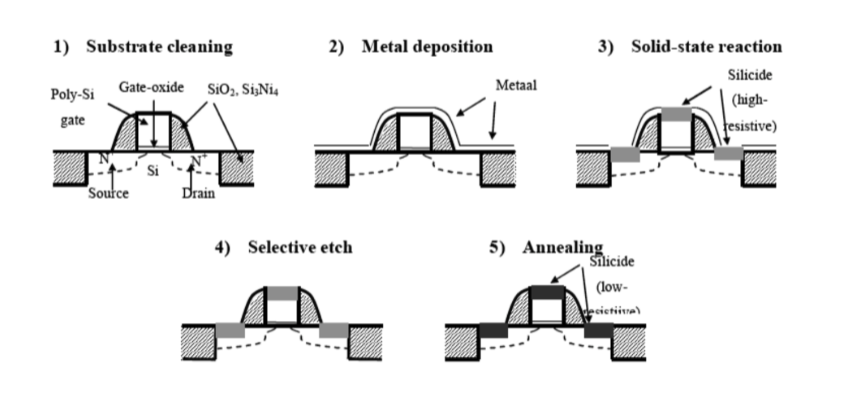
\includegraphics[width=0.5\linewidth]{salicide.png}
    \caption{Salicide}
    \label{fig:enter-label}
\end{figure}

As we get lower and lower, we need to use \gls{ald} to realize this technique.

\begin{figure}[H]
    \centering
    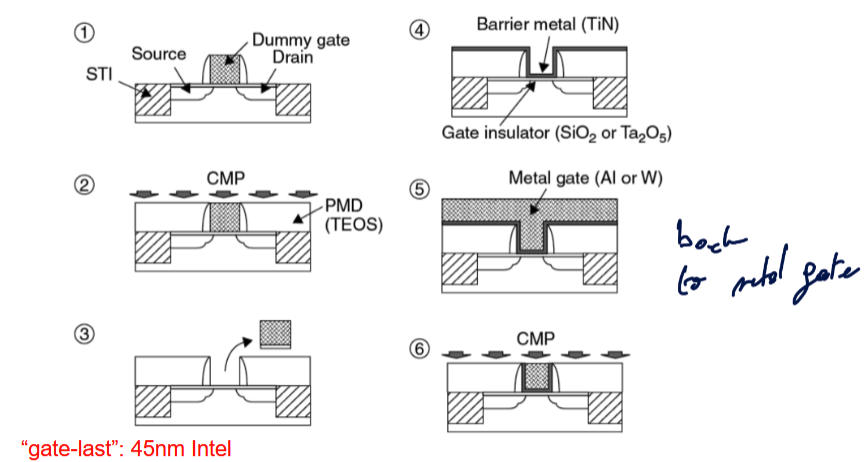
\includegraphics[width=0.5\linewidth]{gate_MOSFET.png}
    \caption{Gate MOSFET}
    \label{fig:enter-label}
\end{figure}



%\chapter{(Chip packaging and PCB process)}
\chapter{Guest Lecture}

% Print all def
\glsaddall

\printglossary[type=\acronymtype, title=Acronyms]
\printglossary[type=definitions, title=Technical Definitions]

\end{document}
